% #############################################################################
% This is Chapter 2
% !TEX root = ../main.tex
% #############################################################################
% Change the Name of the Chapter i the following line
\fancychapter{Background}
% The following line allows to ref this chapter
\label{chap:back}

The development of an algorithmic-based framework for optimization, applicable to architectural domains, requires a careful review over the current literature on \ac{BPO} practices.
	
On the one hand, building design is a multi-disciplinary practice that involves a wide variety of problems that deserve to be optimized. According to their characteristics, some algorithms may be more or less adequate to address them. To maximize the optimization's potential, it is, therefore, necessary to distinguish between different problems and to determine which algorithms are more suitable. Generally, \ac{BPO} practices require the simultaneous optimization of multiple aspects, but this causes performance issues that must be addressed. 
	
On the other hand, the fact that \ac{BPO} requires simulation tools to evaluate the performance of building designs motivates the application of a special class of optimization algorithms, the derivative-free algorithms, as will be described in \cref{sec:optimizationalgorithms}. Within this class, different categories emerge, emphasizing the algorithms' different properties and search strategies. Applying the most adequate algorithms for each problem potentially increases the efficiency of optimization processes, especially for problems involving time-consuming evaluations. 
	
This chapter discusses four different approaches to deal with these problems. After a comprehensive description of the previously mentioned \ac{BPO} practices, in \cref{sec:problemsaddress}, we emphasize their main limitations. 
	
\section{Optimization Problems}
\label{sec:optimizationproblems}	
In simple terms, optimization seeks the set of parameters' values that not only yield the best outcomes in regards to specific criteria, but that also satisfy a set of predefined conditions. Therefore, an optimization process consists in two main parts: the model of the problem to be optimized and the optimization algorithm. This section  will focus on aspects related to the first part, whereas the second part will be discussed in \cref{sec:optimizationalgorithms}.
	
%	Generally, an optimization process consists in two main parts: modeling the optimization problem and executing optimization algorithms. Covered in this section, the first part involves the creation of a model representing the problem to optimize, while the second part, further discussed in \cref{}, focuses on the application of a strategy capable of searching among the set of possible solutions, i.e., the solution space, for the optimal ones.
	
In the mathematical field of optimization, the creation of the model representing the problem to optimize involves the definition of variables, objective functions, and, optionally, constraints \cite{Nocedal2011NumericalOptimization}. In this definition, \textbf{variables} are the parameters whose value will be modified, \textbf{objective functions} represent the performance criteria that we aim to optimize, and \textbf{constraints} are the conditions on the parameters that must be satisfied in order to guarantee that a solution is valid for the defined problem. Given these definitions, most mathematical formulations commonly describe optimization problems through the following set of equations represented in \cref{eq:genericopt}\cite{Koziel2011}, where the $x = (x_1\,, x_2\,, \ldots\,, x_n)$ represents the set of variables, $f_i$ represents the $i$-th objective function (\cref{eq:genericopt1}), and, finally, $g_j$ and $h_k$ represent functions, whose value can be constrained by some conditions in order to guarantee that the obtained solutions are valid (\cref{eq:genericopt2,eq:genericopt3}). 
	
	\begin{subequations}
		\label{eq:genericopt}
		\begin{align}
		\underset{x \in \mathbb{R}^n}{\text{minimize}}
		& \quad f_i(x)\,, &\; i = 1\,, 2\,, \ldots\,, I\,, 
		\label{eq:genericopt1}\\
		\text{subject to}
		& \quad g_j(x) = 0\,, &\; j = 1\,, 2\,, \ldots\,, J\,, \label{eq:genericopt2}\\ 
		& \quad h_k(x) \leq 0\,, &\; k = 1\,, 2\,, \ldots\,, K\,.  \label{eq:genericopt3}
		\end{align}
	\end{subequations}
	
	Optimization has several possible classifications according to the way problems are modeled and to the strategies employed by each optimization algorithm. When considering the formulation of the model, aspects like the variable types, the presence or absence of constraints, and the number and nature of the objective functions can change from problem to problem. Also, the algorithms can be classified differently according to, for example, the determinism of their search, the used information, and the scope of the search, i.e., whether they explore vaster or narrower regions of the solution space. 
	
	Particularly, in \ac{BPO}, building designs may yield different optimization problems, depending on the way they are modeled and the limitations or restrictions imposed by architects or engineers. For example, in order to reduce fabrication costs it is very frequent to limit the granularity of the design's variables. As another example, consider the situation where, to preserve the architect's intention, building designs are confined to have specific shapes (e.g., arc-shaped, round-shaped, squared-shaped). Moreover, it is also possible that when building design becomes more complex, architects decide to relax some of the previously established conditions. Indeed, as it will be further discussed in \cref{ssec:soo,ssec:preferencesarticulation}, when facing problems involving the simultaneous expensive evaluation of multiple performance aspects, time restrictions often force architects to abdicate some performance aspects, or, in some cases, to define a preference amongst the considered performance aspects.
	
\subsection{Problems Classification}
	
	The mathematical optimization field offers different classifications for optimization problems. \Cref{fig:optclassification} presents a schematic representation of the classifications considered in this dissertation. For more comprehensive treatments of these classifications, consider~\cite{Koziel2011, Nocedal2011NumericalOptimization}. 
	 
	The first classification differentiates \textbf{continuous} and \textbf{discrete} optimization problems depending on the variables' types. Continuous optimization refers to problems defined uniquely by continuous variables and, therefore, characterized by an infinite solution space, whereas discrete optimization refers to problems for which some or all their variables are discrete. In continuous optimization, the smoothness of functions makes it possible to reason about the behavior of all points close to a certain point and, consequently, to solve these problems more easily, whilst the commonly present irregularities of discrete optimization functions do not, in general, allow to draw any information about the behavior of points close to a given point. Discrete optimization problems can be subdivided into finer optimization classes, such as integer optimization or combinatorial optimization. 
	% In mathematical analysis, the smoothness of a function is a property measured by the number of derivatives it has that are continuous. A smooth function is a function that has derivatives of all orders everywhere in its domain.
	
	The second classification relates to the presence of constraints on the variables. \textbf{Unconstrained} optimization problems have no restrictions on the variables' values, although they can be penalized for not satisfying certain conditions (called soft constraints). As a consequence, the model of an unconstrained optimization problem is simply represented by \cref{eq:genericopt1}, where each $f_i$ encloses not only the objective functions but also the specified penalties. Conversely, \textbf{constrained} optimization applies to problems where constraints are crucial (e.g., economy problems) and are incorporated into the problem's model using \cref{eq:genericopt2,eq:genericopt3}. Constraints can be hard or soft, depending on whether they must be compulsorily satisfied, or are allowed to be violated. Hard constraints typically correspond to restrictions on the acceptable ranges of values for each variable, such as $-1<x<1$, or to force relations between variables, such as $\sum_{i} x_i<0.5$, whereas soft constraints correspond to the addition of penalties in the objective function, thus worsening the value of the solutions that violate user defined conditions. Constrained optimization problems can be converted to unconstrained ones by replacing hard constraints with soft ones, i.e., by adding penalization terms to the objective function to discourage the violation of constraints~\cite{Nocedal2011NumericalOptimization}. 
	
	The third, and final, classification focuses on the number of objectives to optimize, which can be distinguished into \textbf{single-objective} (\ac{SOO}) and \textbf{multi-objective} (\ac{MOO}). \ac{SOO} focuses on the optimization of one objective, whilst \ac{MOO} focuses on problems involving multiple, possibly conflicting, objectives simultaneously. When modeling an optimization problem using \cref{eq:genericopt}, this difference comes down to the number of objective functions ($I$): $I=1$ for \ac{SOO} problems, and $I>1$ for \ac{MOO} problems. Addressing multi-objective problems entails more complex optimization problems. For problems involving time-consuming evaluations, the increased complexity negatively affects the optimization and spurs the adoption of other, often simpler, approaches. The following sections describe different approaches to single- and multi-objective optimization problems. 
	
	\begin{figure}
		\centering
		\includegraphics[]{Images/Background/classification-opt-problems.pdf}
		\caption{Different classifications of optimization problems.}
		\label{fig:optclassification}
	\end{figure}
	
	% ----------- 
	\subsection{Experimental Approach}
	\label{ssec:doe}
	
	The experimental approach, also known as design of experiments in other fields \cite{Giunta2003DOE}, is widely used in research and in practice to address both single- and multi-objective problems~\cite{Fang2017}. Besides being intuitive and flexible, it can achieve potentially better solutions without having to deal with complex optimization algorithms. This approach evaluates models generated with different values for the parameters, i.e., with different combinations of parameters. These combinations can be obtained through sampling methods, such as \textit{Full Factorial}, \textit{Monte Carlo Sampling}, or \textit{Latin Hypercube Sampling}~\cite{Giunta2003DOE}, which generate different variations of the model to be evaluated. This approach returns multiple solutions instead of just one, leaving the final choice in the hands of the user.
	
	Unfortunately, this approach does not guarantee that good solutions will be found. In fact, in most cases, new solutions are generated without taking advantage of the information obtained from previously evaluated ones. Consequently, the old information is not used to guide the search towards the most efficient solutions and useless candidate solutions can sometimes be evaluated. 
	
	On the other hand, given its simplicity and flexibility, this approach allows architects to easily combine different processes in order to direct the search towards better design solutions. For example, the user can choose a sampling method to generate different design variations, which are then evaluated. After analyzing the results of the evaluations, the user may wish to explore regions of the design space near the most promising design solutions. In that case, he might constrain the design variations to lie within the promising regions, by updating the problem’s definition. The redefined problem is then subsequently sampled and redefined until the user is satisfied with the quality of the obtained solutions.
	
	Despite the constant need for manual intervention, the previous technique can be adapted to automatically extract information about the design problem itself, for example, to study the impact of design parameters in the performance. This process, commonly known as \textit{sensitivity analysis}~\cite{Saltelli2007}, has already been applied in the context of \ac{BPO}~\cite{Tian2013}, not only to achieve better solutions, but also to enhance the performance of existing optimization algorithms, e.g., by dropping irrelevant parameters.
	
	Overall, while it does not provide guarantees about the solutions’ optimality, this approach is simple, easy to use, and it is available in numerous tools. Moreover, although this process is not intelligent \textit{per se}, since the decisions are always made by the user, it enables a more informed design process, as it presents all the design variations generated and their associated performance.
	
	% #############################################################################
	\subsection{Single-Objective Optimization}
	\label{ssec:soo}
	
	\ac{SOO} processes aim to find the best solution with respect to a unique objective function. This function is described in terms of the values of the problem's parameters. \Cref{eq:soo} illustrates an example of a mathematical constrained minimization \ac{SOO} problem, where $f$ represents the single-objective function, $g_j$ and $h_k$ represent the constraints to be satisfied, and $x$ represents the parameters' vector.
	
	\begin{equation} \label{eq:soo}
	\begin{aligned}
	& \underset{x \in \mathbb{R}^n}{\text{minimize}}
	& & f(x) \\
	& \text{subject to}
	& & g_j(x) = 0, & \; j &= 1, \ldots, J, \\ 
	&&& h_k(x) \leq 0, & \; k &= 1, \ldots, K.
	\end{aligned}
	\end{equation}
	
	Generally, the computational complexity of optimization processes is exponential on the number of objectives. In particular, \ac{SOO} processes rely exclusively on a single objective function and are, therefore, usually less time-consuming than \ac{MOO} processes. The main difference between these two processes is that the former focuses on finding the solution that optimizes a single function, whereas the latter focuses on finding the optimal trade-offs between the, potentially conflicting, multiple objective functions. The difference in the computational resources becomes particularly relevant when considering simulation-based objective functions, as these tend to be very time-consuming. 
	
	Particularly, in the case of building design, where most problems include simulation-based objective functions and time is often a limitation, architects commonly opt for \ac{SOO} processes~\cite{Wortmann2017Opossum}: either by simply considering a single performance aspect (or objective), or, in the case of problems involving multiple conflicting aspects, by combining them in a unique function as it will be further explained in \cref{ssec:preferencesarticulation}.
		
	Although \ac{SOO} processes are less time-consuming, these are also less informative than \ac{MOO} processes, as they usually focus on a single optimal solution. As a case in point, building design often involves different conflicting aspects (e.g., thermal comfort, energy consumption, cost), for which information about the different compromises would aid problem comprehension and decision making.
	
	% #############################################################################
	\subsection{\textit{A Priori} Articulation of Preferences}
	\label{ssec:preferencesarticulation}
	
	This approach comprises a simplified way of handling \ac{MOO} that is very resemblant of the \ac{SOO} approach previously discussed, but without disregarding any of the performance aspects. Particularly, this approach combines multiple objective functions according to one’s preferences, using what is called a utility function \cite{Marler2004}, i.e., a function which ranks alternatives according to their utility for global performance. 
	
	Among all the possible utility functions, the most common one is the weighted sum~\cite{Wortmann2017Opossum}, also referred to as \textit{linear scalarization}, in the literature. This utility function reduces \ac{MOO} to \ac{SOO} problems by weighting the different objectives and combining them into a single function, as depicted in~\cref{eq:scalarization}. The weights ($w_i$) assigned to each objective function ($f_i$) represent their relative importance to the architect and they must be set during the modeling of the optimization problem, that is, before starting the search for optimal solutions. The resulting function is then provided to a \ac{SOO} algorithm as the function to optimize. 
	
	\begin{equation} \label{eq:scalarization}
	\begin{aligned}
	& \underset{x \in \mathbb{R}^n}{\text{minimize}}
	& & \sum_{i=1}^n w_i f_i(x), & \; i &= 1, \ldots, n, \\
	& \text{subject to}
	& & g_j(x) = 0, & \; j &= 1, \ldots, J, \\ 
	&&& h_k(x) \leq 0, & \; k &= 1, \ldots, K.
	\end{aligned}
	\end{equation}
	
	Despite its similarity to \ac{SOO}, this approach incurs more computationally complex processes than the latter one, as it involves the evaluation of multiple objective functions. As a result, an utility function evaluation takes as long as the sum of each independent objective function evaluation. Nevertheless, this approach still manages to be less time-consuming than other \ac{MOO} approaches, as it focuses on the optimization of a single combined objective function, instead of attempting to find the trade-offs among all the objectives. 
	
	As a case in point, in architecture, this approach is particularly useful when more experienced architects can use additional knowledge about the problem (e.g., relevance of the different optimization performance aspects) to define an appropriate set of preferences. In terms of the impacts in the design process itself, this approach yields a more intelligent, but less informed design process. On the one hand, it confers intelligence because the involved optimization algorithms exploit the knowledge of previously evaluated solutions to guide the search towards optimal regions of the design space. On the other hand, it is less informed, because architects no longer control or have information about the optimization process. The loss of control results from the automated aspect of the optimization algorithms involved in the architectural practice, which frequently exclude architects from the optimization loop. As a consequence, in general, the architect has no information about the solutions evaluated during the optimization process and is only provided with a single solution~\cite{Custodio2010}. The lack of information is perceived as a limitation \cite{Cichocka2017SURVEY} and it restricts the architect to either comply with the retrieved solution or to rerun the optimization. Either way, this optimization approach does not provide, in general, enough information to understand the optimization results, and, consequently, make more informed decisions. 
	
	% Overall, in architectural domains, the virtues of this approach include the ease of use, the availability, the heterogeneity of ready-to-use \ac{SOO} tools (e.g., Opossum, Goat, Galapagos, Silvereye), and the time complexity. %when compared to other \ac{MOO} approaches. % In general, because this preference-based approach focus in the retrieval of a single optimal solution that satisfies the previously defined preferences, it becomes more effective and less time consuming than other \ac{MOO} approaches, that either lack a more guided search or that aim at finding solutions that are optimal under different preference articulations. 
	% #############################################################################
	\subsection{Pareto-based Optimization}
	\label{ssec:pareto}
	
	Despite allowing users to handle \ac{MOO} problems, the previous approach does not consider the different trade-offs among the potentially conflicting objectives, instead forcing users to make an \textit{a priori} decision regarding the importance of each objective. Pareto-based optimization approaches attempt to address this limitation by postponing that decision until the end of the optimization process. In this approach, all objectives are taken as equally important during the optimization, making it more difficult to discern the quality of each solution. In other words, while in \ac{SOO} problems we expect the optimal solution to be the configuration that achieves the best\footnote{For simplification purposes, we simply refer to the optimal solution as being the best. When dealing with a minimization problem, the best solution is the one that achieves the lowest value of the objective function, whereas in maximization problems, the best solution is the one achieving the highest value of the objective function.} objective value possible, in \ac{MOO}, the best configuration for one of the objectives is rarely the best possible one for all other objectives, which results from the fact that these objectives are often conflicting. \Cref{eq:pareto-based} presents an example of the mathematical definition of a constrained minimization \ac{MOO} problem, where $F(x)$ represents the vector of $m$ objectives, $f_i$ represent the $i^{th}$ objective function, $g_j$ and $h_k$ represent the constraints to be satisfied, and $x$ represents the parameters' vector.
	
	\begin{equation} \label{eq:pareto-based}
	\begin{aligned}
	& \underset{x \in \mathbb{R}^n}{\text{minimize}}
	& & \left\lbrace F(x) = \left[f_1(x), f_2(x), ..., f_m(x)\right]  \right\rbrace \\
	& \text{subject to}
	& & g_j(x) = 0, & \; j &= 1, \ldots, J, \\ 
	&&& h_k(x) \leq 0, & \; k &= 1, \ldots, K.
	\end{aligned}
	\end{equation}
	
	In order to assess the quality of multi-objective solutions, it becomes necessary to apply a new optimality criterium, like the Pareto optimal (or Pareto efficient) concept. Named after the economist Vilfredo Pareto, the Pareto optimal concept defines an optimal solution as being a solution for which it is impossible to improve an objective value without deteriorating others. Such a solution is also said to be nondominated or noninferior, and the set of nondominated solutions is called the Pareto front. An example of a bi-objective minimization problem is illustrated in \Cref{fig:paretofrontier}. The two objectives are $f_1$ and $f_2$, and the solutions shown in orange are nondominated. The goal of Pareto-based optimization algorithms is to find design solutions that lie on the Pareto front.
	
	% Begin Pareto-Optimization Figure -------------------------------------------------------
	\begin{figure}
		\centering
		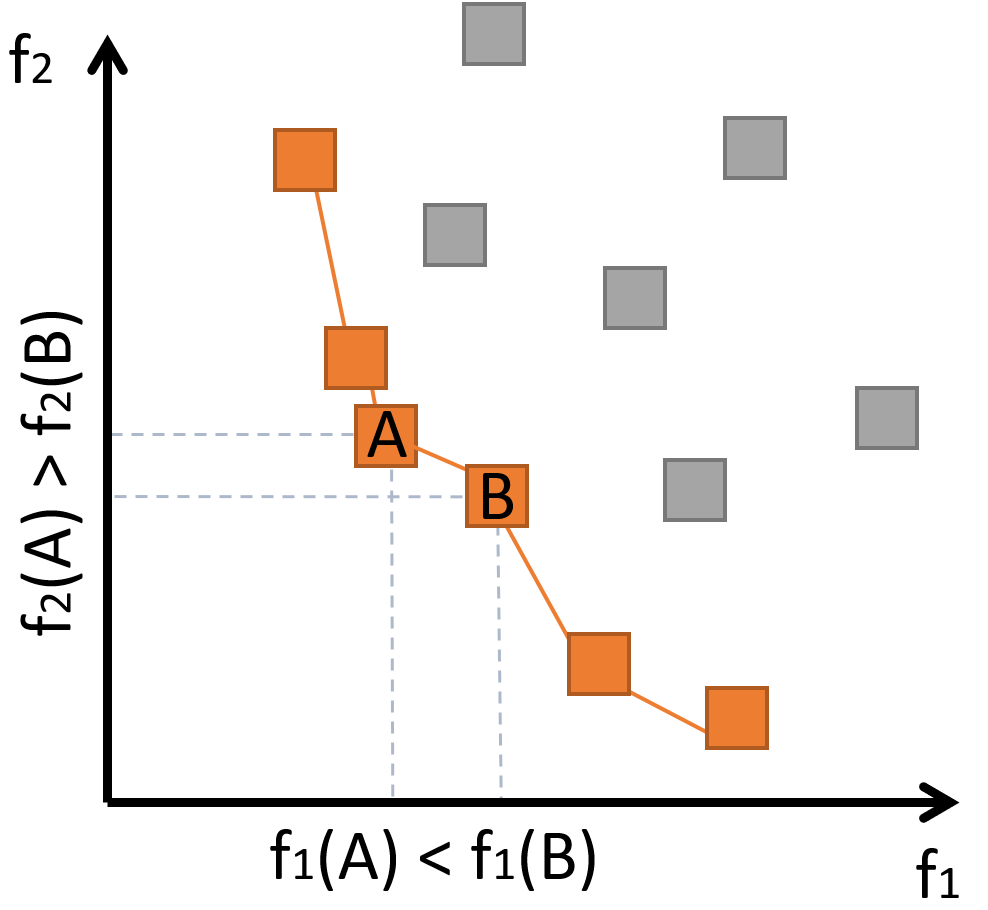
\includegraphics[width=0.35\textwidth]{Images/Background/pareto-front.PNG}
		\caption[Representation of a Pareto front example for a bi-objective optimization problem]{Representation of the set of nondominated (orange squares) and dominated (gray squares) solutions for a bi-objective minimization problem. The Pareto front is composed of all the nondominated solutions.}
		\label{fig:paretofrontier}
	\end{figure}
	% End Figure -------------------------------------------------------
	
	When considering the architectural practice, building design is a complex task that frequently involves dealing with multiple conflicting objectives, such as maximum lighting comfort \textit{versus} maximum thermal comfort, or minimum energy consumption \textit{versus} maximum thermal comfort. Even though the three previous approaches provide enough mechanisms for handling \ac{MOO} problems, they lack a more guided and informative strategy capable of retrieving a diverse and representative set of different trade-offs between the various performance aspects, i.e., the objective functions.
	
	Alternatively, the Pareto-based optimization approach provides the user with the set of nondominated solutions that represent the different conflicts or trade-offs between the considered objectives. When confronted with these solutions, architects can compare the different design options according to different performance criteria, and, thus, make more informed decisions about the different compromises involved. 
	
	On the other hand, in this approach, (1) the number of function evaluations is larger due to the need to find a set of optimal solutions instead of focusing on a single one, (2) the visual representation of the values of the solutions' objectives becomes problematic when the number of objectives is greater than three, and (3) the way the optimization problem is modeled has a direct impact on the quality of the solutions.
	
	% #############################################################################
	\subsection{Comparison}
	\Cref{table:optapproach} shows a comparison between the optimization approaches mentioned in this chapter and discusses their applicability in the context of architectural practice.
	 
	On the one hand, in terms of manual intervention, the experimental approach confers higher levels of control at the cost of constant manual intervention (e.g., number of variations to generate, number of iterations to run sampling methods, choice of optimal solutions). The same does not happen with other approaches for which intervention is residual or even inexistent.	
	
	On the other hand, with higher control levels, the user gains more insight about the optimization process. Concretely, when following an experimental approach, the user is provided with all the information about all the solutions that were evaluated during the optimization process, whereas in the other approaches the user is only provided with the optimal solutions. The availability of information has a direct impact in the ability to comprehend the optimization results.
	\begin{table}
		\centering
		\caption{Comparison between different optimization approaches.}
		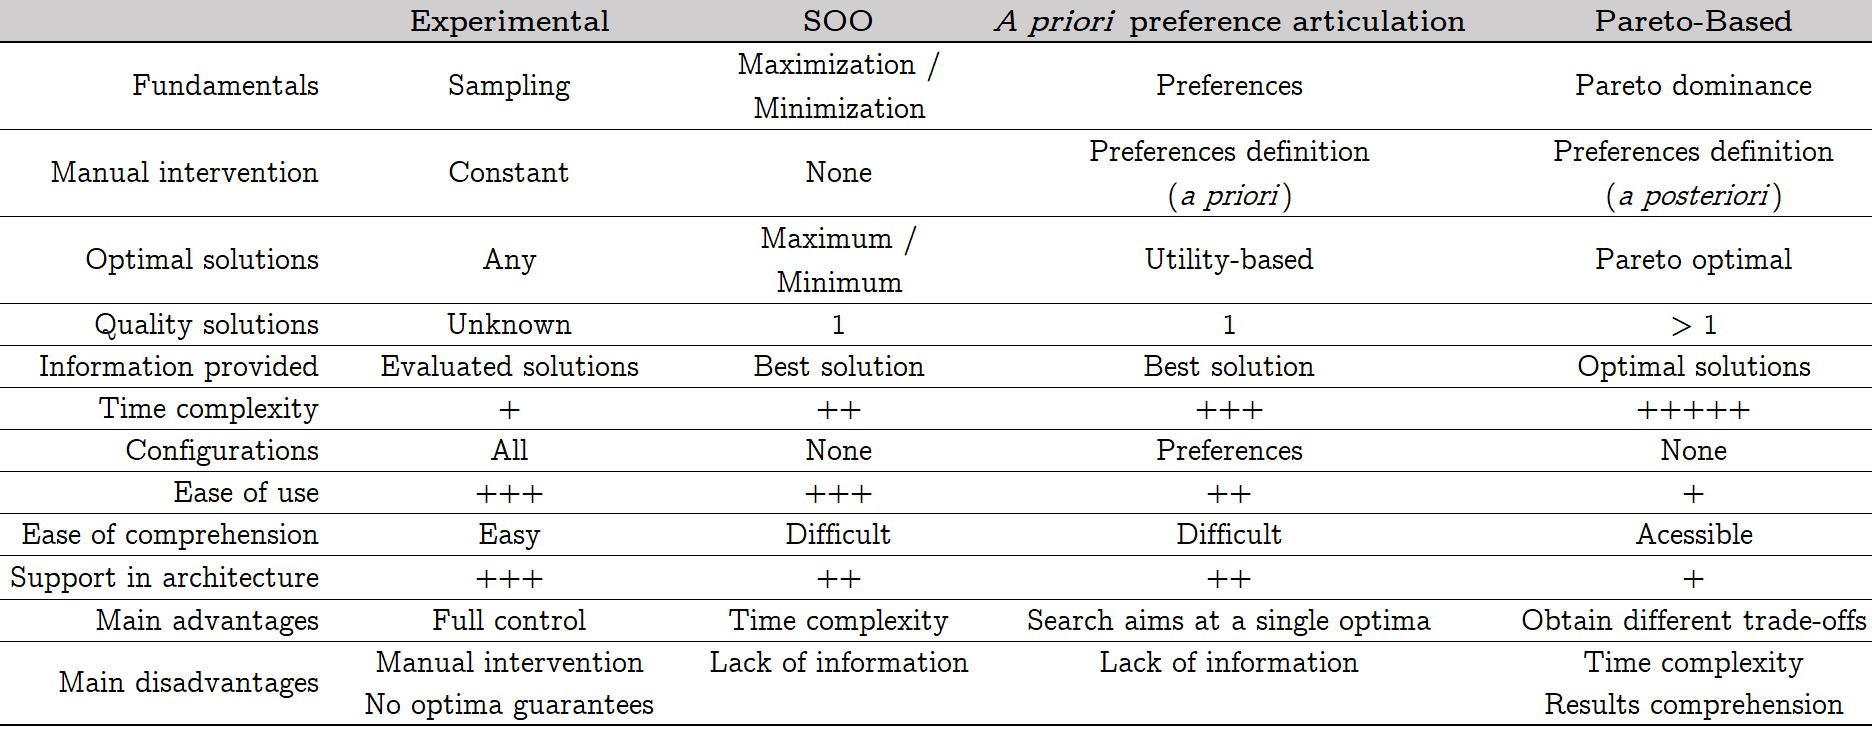
\includegraphics[width=1\textwidth]{tables_and_code/approaches_comparison.PNG}
		\label{table:optapproach}
	\end{table}

	The automation of optimization processes prompts the need for automatically evaluating the quality of solutions, thus requiring some optimality concepts: (1) depending on whether it is a maximization or a minimization problem, the \ac{SOO} approach considers the best solution to be the one presenting the largest or smallest value, respectively; (2) the \textit{a priori} preference of articulations approach applies a similar criteria, but it first entails the definition of a utility function to reduce a \ac{MOO} to a \ac{SOO} problem; and (3) the Pareto-based optimization approach is based on Pareto optimality, leaving the final decision about the optimal solutions to the user.
	
	Depending on the approach, the number and quality of solutions may vary. In general, all but the experimental approach presents a guided and, thus, more intelligent strategy to seek efficient solutions. As a result, that approach does not guarantee that good solutions are found. Conversely, the other approaches tend to yield one or more (near) optimal solutions depending on whether or not they are Pareto-based.
	
	A crucial point to take into consideration is the time difference between each approach, with the Pareto-based and the experimental approaches being the most and the less time-consuming, respectively. The former requires searching the solution space with the aim of finding the best trade-offs between different objectives, whereas the latter simply relies on a sampling strategy which generates different variations of parameters to be evaluated. This time difference is particularly concerning in the case of problems with costly evaluation functions, as it is the case of building design. Even though the \textit{a priori} preference-based approach involves the same objectives as the analogous Pareto one, it can be considerably faster. This results from the fact that this approach focuses on the satisfiability of a certain set of preferences, instead of exploring a wider set of solutions.
	
	Indeed, when focusing on architecture, Pareto-based approaches are less applied in practice. Nevertheless, a few studies concerning this optimization approach have emerged in the past years, evidencing its utility~\cite{Evins2013,Hamdy2016}. Additionally, recent works show that despite the lower time complexity of \ac{SOO}-based and \textit{a priori} preference-based approaches, they are not as desirable as the Pareto-based ones, which can be explained by the benefits of Pareto-based approaches to the decision making process~\cite{Attia2013,Cichocka2017SURVEY}. %Moreover, these multiple compromises represent different articulation of preferences from which the architect selects one. This approach is also called \textit{a posteriori} articulation of preferences.

	Despite the growing interest and the notable increase in works featuring optimization in \ac{BPO}, most of them fall into the same class of algorithms~\cite{Evins2013,Nguyen2014}. Moreover, the majority of studies tend to focus on \ac{SOO} problems and do not provide any relevant conclusion about \ac{MOO} problems within \ac{BPO} practices. The prevalence of \ac{SOO} practices might be explained by a few factors. Firstly, single-objective problems are easier to model. Secondly, common optimization tools in architecture, like Galapagos and Goat, allow users to easily address single-objective \ac{BPO} problems. As a result, not only are architects capable of solving these optimization problems, but, when facing more complex \ac{MOO} problems, they are also encouraged to adopt simplified versions of such problems, thus reducing the overall complexity of the optimization processes. Finally, the wider variety of optimization algorithms exposed in \ac{SOO} plug-ins enables the selection of the best algorithm to specific problems, thus spurring more efficient optimization processes~\cite{Wortmann2016BBO}.  
	
	Nevertheless, \ac{BPO} often involves design problems with multiple conflicting aspects (e.g., thermal comfort, lighting comfort, energy consumption, cost). Therefore, the studies of \ac{MOO} approaches, including the Pareto-based ones or the \textit{a priori} articulation of preferences, is of great importance for architecture. Despite the recent growing trend of these approaches\cite{Evins2013,Wortmann2017Opossum}, the number of relevant benchmarks comparing the performance of such algorithms is still very small and unclear about the best practices and the behavior of the algorithms for \ac{BPO}.  
	%Each optimization approach comprises different optimization algorithms. In the particular case of building design, the nature of the costly evaluation functions not only directly influences the overall optimization time, but also the algorithms' nature, as discussed in the following section. 
	%Overall, in architectural domains, the virtues of this approach include the ease of use, the availability, the heterogeneity of ready-to-use \ac{SOO} tools (e.g., Opossum, Goat, Galapagos, Silvereye), and the time complexity. %when compared to other \ac{MOO} approaches. % In general, because this preference-based approach focus in the retrieval of a single optimal solution that satisfies the previously defined preferences, it becomes more effective and less time consuming than other \ac{MOO} approaches, that either lack a more guided search or that aim at finding solutions that are optimal under different preference articulations. 
% ##########################################################################
% ##########################################################################

% ##########################################################################
\section{Optimization Algorithms}
\label{sec:optimizationalgorithms}
	Optimization processes are comprised by two parts: the first one, previously described, focuses on the modeling of the problem; the second one involves exploring different values for the set of variables defined in the model with the aim of finding more efficient solutions. This exploration part is achieved by means of optimization algorithms, which will be the focus of this section. 
	
	All optimization algorithms seek optimal solutions in the solution space. However, each algorithm exploits different techniques to enhance its search process, which causes some algorithms to outperform others in some types of problems \cite{Wolpert1997NFLT}.
	
	In order to identify which algorithms are more appropriate for specific optimization problems, it is necessary to measure their quality. Whereas this is rather straightforward for \ac{SOO} algorithms, the same does not happen for \ac{MOO} algorithms, as it will be discussed in \cref{ssec:performance}.
	
	\subsection{Algorithm Classification}	
	Mathematically speaking, optimization algorithms can be classified differently according to their properties. \Cref{fig:optALGOclassification} presents a schematic representation of the classifications considered in this dissertation. For a more comprehensive treatment of these classifications, we refer the reader to \cite{Koziel2011, Nocedal2011NumericalOptimization}.
	
	One important classification regards the extent of the search for optimal solutions, which can be \textbf{global} or \textbf{local}. Local optimization algorithms strive to find a locally optimal solution, i.e., for which the objective function yields a better value than for all the other solutions in its vicinity. Moreover, local algorithms are usually highly sensitive to the starting point of the search and they tend to focus on smaller regions of the solution space. In contrast, global optimization algorithms strive to find globally optimal solutions, i.e., the best of all the locally optimal solutions. To that end, these algorithms explore larger regions of the solution space and typically require several evaluations to find global optima. However, the increased number of evaluations can be problematic in problems involving expensive objective functions. To minimize this impact, a good approach might be to apply a global algorithm to identify a promising region and then apply a local algorithm to more rapidly find the optima within that region. 
	
	
	\begin{figure}
		\centering
		\includegraphics[]{Images/Background/classification-opt-algorithms.pdf}
		\caption{Different classifications of optimization algorithms.}
		\label{fig:optALGOclassification}
	\end{figure}
	
	A second classification differentiates \textbf{deterministic} and \textbf{stochastic} algorithms depending on the determinism of the algorithms' outcomes. Given the same starting point and configuration, deterministic algorithms systematically apply the same sequence of steps and, as a consequence, they always return the same result. In contrast, stochastic algorithms include some form of randomness within their description and, therefore, often yield different results for the same starting point and algorithm's configuration.
		
	The third, and final, distinction is between \textbf{derivative-based} and \textbf{derivative-free} algorithms, which differ in the type of information used during the search. Derivative-based (or gradient-based) algorithms explore information from the derivatives of objective functions, i.e., the direction and magnitude of the greatest increase of the function, to guide the search. % Consequently, they solve problems explicitly defined through mathematical forms very efficiently, as the derivatives' information is easily available. 
	However when the objective function's analytical form is unknown and the derivatives are unavailable, these algorithms cannot be applied. Although finite-difference methods could be applied to approximate the derivatives, these require several extra function evaluations, which becomes impractical for problems involving expensive objective functions. In these cases, it becomes necessary to resort to derivative-free algorithms, which, instead of exploiting information about derivatives, treat the objective functions as \textit{black-boxes} and use the result of previously evaluated solutions to guide the search~\cite{Rios2013}.
	
	Derivative-free optimization algorithms, commonly known as black-box optimization algorithms within the architectural community \cite{Wortmann2016BBO},
	can treat the results of performance simulations as the functions to optimize and, consequently, avoid the difficulty of deriving analytical formulas describing building performance \cite{Machairas2014}.
	
	For the past decades, the constant development and improvement of derivative-free optimization resulted in the creation of algorithms with different underlying assumptions and different properties. Although there is no standardized classification for these optimization algorithms~\cite{Rios2013, Wortmann2017ADO}, it is possible to group them according to their main mechanisms and ideas. This dissertation follows the classification proposed in the context of architectural design~\cite{Wortmann2015AdvSBO}, which first subdivides the algorithms according to the search strategy's determinism, namely, metaheuristics and iterative methods, and only then proceeds to partition the latter into direct-search and model-based methods, based on the function explored to guide the search. Albeit the apparent chasm between these classifications, some algorithms draw ideas from distinct classes, thus emphasizing not only the blurred lines of such categorizations, but also the difficulties that lie within the definition of more standardized classifications. 
	
	The following subsections describe the classes of algorithms that will be explored in this dissertation, including sampling algorithms and the three classes of derivative-free algorithms: direct-search, metaheuristics, and model-based. Additionally, a summarized explanation of some of the most relevant algorithms will also be provided. For more extensive explanations, we suggest \cite{Tille2006} for sampling algorithms, \cite{Conn2009} for direct-search algorithms, \cite{BlumRoli2003Metaheuristics, Glover2003Metaheuristics, Zhou2011} for metaheuristic algorithms, and \cite{Koziel2011} for model-based algorithms.
	
	\subsection{Sampling Algorithms}
	\label{ssec:sampling}
	In general, sampling algorithms select a subset of a population, called samples. In the case of an optimization problem, a population generally consists of all the possible solutions, i.e., all the possible combinations for the values of the variables that satisfy the modeled constraints. In this case, the samples would be the subset of all the possible solutions and the sampling algorithm would be the strategy for selecting this subset. Despite being simple, and easy to implement, these strategies focus on the solutions' distribution and do not take into account the results of previous objective function evaluations. As a consequence, sampling algorithms cannot be considered true optimization algorithms. Instead, they should only be used as an initial approach or as an internal step of an optimization algorithm.
	
	There are several interesting examples of sampling algorithms \cite{Tille2006}. The simplest one, called \textit{Monte Carlo} (or \textit{Random}) \textit{sampling}, consists on a random selection from the population, which often leads to large gaps of unexplored possibilities. Increasing the samples' size might help circumventing this limitation, but a better approach is to use the \textit{Latin Hypercube sampling} algorithm, especially when dealing with computationally complex objective functions. In particular, this algorithm subdivides the space into equally sized bins and randomly chooses a solution within each bin. Besides requiring less samples, this algorithm ensures a better distribution of the samples.
	
	In the particular case of architecture, sampling algorithms are typically used in the context of experimental approaches, as discussed in \cref{ssec:doe}. In these cases, sampling algorithms are used to generate different design variations, which are then evaluated using the analysis tools. In the end, architects select the solutions that better satisfy their needs.
	
	% ----------- Subsection
	\subsection{Direct-search Algorithms}
	\label{ssec:direct-search}
	
	Although there seems to be no precise definition for direct-search algorithms, these are often identified as algorithms that iteratively: (1) evaluate a sequence of candidate solutions, proposed by a deterministic strategy; and (2) select the best solution obtained up to that time \cite{Conn2009}. Direct-search algorithms are sought as valuable tools to address complex optimization problems, not only because most of them were proved to rely on solid mathematical principles, but also due to their good performance at initial stages of the search process~\cite{Rios2013}. 
	
	% Their slow asymptotic convergence are because they usually using gradient information. Another limitation that is not evident from this example is that the algorithm may be slow to converge if the level sets of f are extremely elongated. This is because the method makes no use of curvature information, the asymptotic rate of convergence will be slow.
	The main limitations of these algorithms is their performance deterioration with the increase on the number of input variables, and their slow asymptotic convergence rates as they get closer to optimal solutions~\cite{Kolda2003}. Moreover, despite the existence of algorithms and benchmarks comparing SOO direct-search algorithms \cite{Waibel2018}, only recently have these started to appear in the context of MOO \cite{Custodio2010}. 
	
	Undoubtedly, one of the most relevant direct-search algorithms is the NMS \cite{Nelder1964}. \textit{\ac{NMS}} is a local \ac{SOO} direct-search algorithm that exploits a simplex to guide the search towards a locally optimal solution. The \textit{\ac{NMS}} algorithm envelopes a region of the design space using a simplex, which is a generalization of a triangle to arbitrary dimensions, i.e., a triangle in two dimensions, a tetrahedron in three dimensions, etc. The simplex is then successively modified using operations, like reflection, expansion, contraction, and shrinking, that iteratively replace the simplex's worst vertex values. % http://www.scholarpedia.org/article/Nelder-Mead_algorithm
	Unlike other direct-search algorithms, \textit{\ac{NMS}} requires no more than two function evaluations per iteration, except when applying the shrinking operation. The initial simplex highly influences the performance of the algorithm: while smaller initial simplices often lead to local searches that converge towards a local optimum, larger initial simplices allow the algorithm to cover a larger extent of the solution space, thus becoming more robust to local optima.
	
	Another interesting simplex-based algorithm is \textit{SUBPLEX} \cite{Rowan1990}, which attempts to overcome the \textit{\ac{NMS}} difficulties when addressing higher dimensional problems by decomposing the problem in low\nobreakdash-\hspace{0pt}dimensional
	subspaces. To that end, \textit{SUBPLEX} subdivides the design space in low-dimensional subspaces and then applies the \textit{\ac{NMS}} algorithm to the most promising subspaces, in order to seek for a better solution. %In contrast to \ac{NMS}, which has difficulties in high-dimensional problems, \textit{SUBPLEX} reduces the limitations through the decomposition of the problem in low-dimensional subspaces which are more efficiently optimized by \ac{NMS}.
	In the same vein, \textit{\ac{PRAXIS}} \cite{Brent1973} also decomposes the problem in smaller ones, by considering each dimension of the solution space separately. Concretely, \textit{\ac{PRAXIS}} moves from one solution to another by iteratively finding better solutions in every other dimensions and then combining them into a candidate solution. 
	
	Besides the local algorithms discussed so far, \textit{\ac{DIRECT}} is a very promising global algorithm. \textit{\ac{DIRECT}} \cite{Jones1993DIRECT} is a \ac{SOO} algorithm which recursively subdivides the design space into smaller multidimensional hyper-rectangles, each represented by a solution in their centre. For each solution, the objective function is evaluated, thus yielding an estimate of the quality of each rectangle. Based on these values, \textit{\ac{DIRECT}} focus the search on more promising regions of the design space, further subdividing those. To minimize the overall number of function evaluations, \cite{Gablonsky2001} suggested a modification to \textit{\ac{DIRECT}} to make it more efficient for functions with few local optima and a single global optimum. This modified algorithm, called \textit{\ac{DIRECT}-L}, differs from the original one by grouping the hyper-rectangles based on the size of the longest rectangle side and by allowing at most one subdivision in each group, i.e., at most one hyper-rectangle of each group can be subdivided in each iteration. These modifications to the original algorithm promote the reduction of the number of divisions, which has a direct impact on the overall number of function evaluations.
	
	\textit{\ac{DMS}} \cite{Custodio2010} is a global multi-objective direct-search algorithmic framework which combines the main ideas of directional direct-search algorithms with the Pareto dominance concepts. In simple terms, \textit{\ac{DMS}} maintains a list of feasible nondominated solutions and their associated step sizes. Then, it iteratively selects nondominated solutions from this list and evaluates a few solutions along a predefined set of directions located at a distance determined by the solution's step size. If during the exploration better solutions are found, then the list is updated. On the other hand, if no better solutions are found, the associated step size is reduced. The process then repeats. This algorithmic framework extends to \ac{MOO} the directional type direct-search algorithms, such as pattern search \cite{Kolda2003}, among others. 
	
	% \Cref{appendix:AlgorithmsDefinitions} provides a more complete description of these and other direct-search algorithms, including SUBPLEX, PRAXIS, and DIRECT-L, among others.	the global algorithm MultiGLODS.
	Overall, direct-search algorithms are not as popular as other classes of derivative-free algorithms. Nevertheless, its convergence proofs and the recent developments in the field of \ac{MOO} make this class very appealing for \ac{BPO}. 
	
	% ----------- Subsection
	\subsection{Metaheuristics Algorithms}
	\label{ssec:metaheuristics}
	In the original definition, these algorithms were solely based in the interaction between local improvement procedures, called heuristics, and higher-level strategies, called metaheuristics. On the one hand, heuristics are techniques that locate good solutions, but not necessarily the optimal, nor the correct ones, and that often consider the trade-off between precision, quality, and computational effort. On the other hand, a metaheuristic is an algorithmic framework that can be applied to different problems, with few modifications to add problem-specific knowledge, if so desired~\cite{Glover2003Metaheuristics}. Moreover, a metaheuristic is a higher-level strategy that extends the capabilities of heuristics by combining one or more heuristic methods, while being agnostic to each heuristic. The ``meta'' classification of these algorithms results from the fact that they control the heuristics applied in the process.
	
	%Throughout time, this class has grown to include any algorithm that includes simple heuristics to locate good solutions in complex design spaces.%, while considering the trade-off between precision, quality, and computational effort of the solutions. 
	These algorithms often rely on randomization, and biological or physical analogies, to perform robust searches and escape local optima~\cite{Glover2003Metaheuristics}. Additionally, their stochastic nature confers them the ability to effortlessly handle complex and irregular objective functions, to adapt to \ac{MOO} contexts, or to provide domain-specific knowledge through heuristics \cite{Wortmann2017GABESTCHOICE}.
	
	Metaheuristics are good optimization algorithms when provided with sufficient amounts of time to do the necessary objective function evaluations \cite{Conn2009}. However, in some contexts, this is not possible. This is the case of \ac{BPO} in the architectural practice, where each evaluation is so time-consuming that the execution of thousands of evaluations rapidly becomes an infeasible scenario. Due to their stochastic nature, limiting the number of evaluations has severe repercussions on their convergence guarantees \cite{Hasancebi2009}.
	
	Depending on the metaphors adopted by each algorithm, metaheuristics can be classified in different subclasses, including, among others, \acp{EA}, which explore Darwinian natural selection and evolution concepts (e.g., heredity, reproduction, genes, recombination, crossover, and mutation), Swarm algorithms, which explore collective intelligence through the cooperation of homogeneous agents in the environment (e.g., birds, ants, bees), and Physical Algorithms, which take inspiration from physical processes (e.g., the annealing process in metallurgy) \cite{Brownlee2011}.
	
	The \textit{\ac{GA}} is undoubtedly one of the most popular metaheuristics algorithms. As an \ac{EA}, it explores the mechanisms of biological evolution to search for better solutions. In particular, it randomly generates an initial set of individuals representing the candidate solutions, called population, which is then evolved for a specified number of iterations (or generations). The evolution process is comprised of four main phases: (1) adaptability, where individuals of the population are assigned a suitability or fitness value; (2) mating selection, where pairs of individuals are selected for reproduction, based on a probabilistic function which is usually proportional to each individual's fitness value; (3) crossover, where the genotypes of the selected individuals are recombined to produce new individuals; and (4) mutation, where new individuals are subjected to random copying errors with a certain probability. While in earlier generations, populations are usually more diverse, in final generations, their individuals are often very similar to the fittest individuals, i.e., we observe an intensification of the traits of the most suitable individuals, thus emulating the natural selection mechanism \cite{Brownlee2011}. % Besides genetic algorithms \cite{Golberg1989,Holland1992}, evolutionary algorithms encompass other algorithms such as Genetic Programming~\cite{Koza1992}, Evolution Strategies \cite{Schwefel1981}, Differential Evolution \cite{Storn1997}, among others. 
	
	Along the same line, \textit{\ac{NSGA-II}} is a \textit{\ac{GA}} specially tailored for \ac{MOO} problems, which incorporates the ideas of population genetics and evolution, Pareto dominance, and a crowding measure to attain an approximation of the Pareto front that is both accurate and diverse \cite{Deb2002}. In simple terms, \textit{\ac{NSGA-II}} maintains an archive and a population, which are iteratively evolved until a stopping criteria is met. Every iteration, the algorithm combines the archive and the population and sorts their individuals according to their nondomination ranks, a measure of the number of Pareto fronts that have to be removed until an individual becomes nondominated. The individuals belonging to the same rank are also sorted according to a density measure, based on the average distance of their two closest individuals. Afterwards, the archive is replaced with the best $50\%$ individuals binary tournaments, i.e., a selection strategy that compares pairs of individuals and selects the best one, which are then carried out on the archive to generate the next offspring population. 

	Besides \textit{\ac{NSGA-II}}, \textit{\ac{SPEA2}} is also a widely reputed \ac{MOOA} \cite{Zitzler2001SPEA2}. As an \ac{EA}, it incorporates evolutionary mechanisms to incrementally evolve a population from generation to generation. In addition to the population, \textit{\ac{SPEA2}} maintains a set of optimal solutions called archive. Initially, the archive is filled with nondominated individuals and, if insufficient, with dominated ones. Then, while a stopping criteria is not met, in every iteration, each member in the population is ranked according to the number of solutions it dominates and to a crowding measure based on the inverse of the distance to the $k^{th}$ nearest neighbor, where $k$ has been previously specified. 
	% \footnote{The density metric is an adaptation of the $k^{th}$-nearest neighbor method. For each individual in the population and archive, compute the pairwise distances to the other individuals and store them in a list. Then sort the list and pick the $k^{th}$ element, where $k$ is commonly set to be the square root of the list size~\cite{Zitzler2001SPEA2}.}
	Then, based on these rankings, the best individuals are continuously incorporated into the archive, removing any dominated solution by them. In the event of surpassing the archive's size, the algorithm also removes individuals that lie in more crowded regions of the nondominated front using a clustering technique. Finally, binary tournaments are carried between elements in the archive and in the population to select the individuals for reproduction, in order to create offsprings for the next generation. These individuals result from the recombination and mutation of the best individuals from the previous generation. 
		
	In addition to \acp{EA}, other metaheuristic algorithms have also been successfully applied to address optimization problems. One example is \textit{Simulated Annealing}, a Physical Algorithm. Resemblant of \textit{Stochastic Hill Climbing} algorithms, where new candidate solutions are randomly sampled and accepted if they represent an improvement, this algorithm iteratively re-samples the solution space aiming at finding an optimal solution. However, in contrast to those algorithms, the \textit{Simulated Annealing} algorithm may accept re-sampled solutions with lower performance, according to a probabilistic function that becomes more discerning of the quality of the samples as the number of iterations increases, thus resembling the natural annealing process \cite{Brownlee2011}. 
	
	Although less explored, \ac{PSO} algorithms, such as \textit{OMOPSO} and \textit{SMPSO} \cite{Sierra2005OMOPSO,SMPSO}, have also been shown to yield promising results in some optimization problems, even surpassing some of the most reputed \acp{EA} \cite{Durillo2011SMPSO}. In their simpler versions, \ac{PSO} algorithms are global algorithms inspired by biological systems, such as the collective behavior of flocking birds or fish schooling, which interact and learn from one another to solve problems. In \ac{PSO}, the intelligence is decentralized, self-organized, and distributed throughout the participating particles, also known as swarm. These particles maintain information about their velocity, their current and personal best positions, and also the global best position known to the swarm. At each time step, the position and velocity of each particle are updated according to the best swarm or close neighbor position~\cite{Brownlee2011}.
	
	Besides these algorithms, it is also possible to find other interesting metaheuristics algorithms in the literature \cite{Zavala2014, Wortmann2017GABESTCHOICE}, including $\epsilon$\textit{-MOEA} \cite{Deb2003EpsMOEA}, \textit{MOEA/D} \cite{Zhang2007MOEAD}, \textit{PESA2} \cite{Corne2001}, \textit{ESCH} \cite{Santos2010}, \textit{ISRES} \cite{Runarsson2000}, \textit{CMA-ES} \cite{Hansen2006}, \textit{PAES} \cite{Knowles1999}, \textit{GDE3} \cite{GDE3}, and \textit{CRS2} \cite{Kaelo2006CRS2}, among others.
	
	Overall, metaheuristics are stochastic algorithms, mostly without convergence guarantees, usually requiring several hundreds or even thousands of evaluations in order to obtain good solutions. For problems involving expensive objective functions, like \ac{BPO}, these algorithms are usually not a good choice. Their overall time complexity becomes even more concerning in the case of \ac{MOO}, as the number of objectives increases. Unfortunately, there is a predominance of these algorithms (e.g., \textit{\ac{GA}}, \textit{\ac{SPEA2}}, and \textit{\ac{NSGA-II}}) among \ac{BPO} practitioners \cite{Wortmann2017GABESTCHOICE}, with very few tools providing support for other classes of algorithms. Nevertheless, they present several parameters that can be fine-tuned to improve their performance and, in fact, they can be very efficient solvers when properly configured. However, the optimal set of parameters is problem-specific and the same configuration applied to another problem might yield a bad performance.
	
	\subsection{Model-based Algorithms}
	\label{ssec:model-based}
	Model-based algorithms are effective handlers for problems characterized by the large time complexity associated with the computation of the objective function and by the absence of information about the objective function \cite{Forrester2009SBO}. Model-based algorithms are able to provide faster estimates of a design’s performance, by supplementing or replacing the original objective function with an approximation \cite{Wortmann2016BBO}. This approximation, called the surrogate, is generated from a set of known objective function values and is then explored to determine the promising candidate solutions to evaluate next. The results obtained from evaluating the candidate solutions are then used to improve the surrogate and this process is repeated until a stopping condition is satisfied \cite{Koziel2011}.
	
	Despite having a well-defined analytical form, which makes computations on the surrogate model more efficient than on the original objective function, the surrogate is only an approximate representation of the original function, and, therefore, must be constantly updated to guarantee a reasonably accurate local representation~\cite{Koziel2011}. \Cref{fig:sbosexample} illustrates a surrogate that is reasonably accurate near the initial solutions. However, as we analyse solutions far from the initial ones, the accuracy of the surrogate model worsens.
	% Begin Figure: SBO Simple Example ----------------------------
	\begin{figure}[h!]
		\centering
		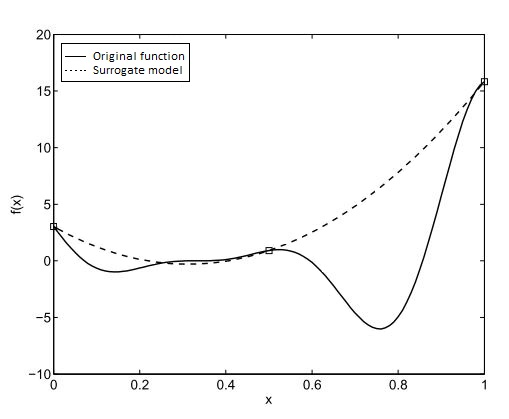
\includegraphics[width=8cm]{Images/Background/sbosexample.JPG}
		\caption[Example of a surrogate model]{Original function and corresponding surrogate model, created based on three initial solutions (squares). This image was retrieved from~\cite{Koziel2011}.}
		\label{fig:sbosexample}
	\end{figure}
	% End Figure -------------------------------------------------------
	
	Nowadays, the techniques applicable to the generation of surrogate models range from trust-region methods to \ac{ML} techniques. These techniques can be used to create (1) local surrogates, i.e., models where the approximation to the objective function is built around a certain point, and (2) global surrogates, i.e, models where the approximation is generated from all the obtained points. Whilst the former relies on the construction of simple, partial models of the objective function, the latter relies on the creation of a full model, which requires balancing the need for improving the model's accuracy by exploring broader regions in the solution space with the need for improving the objective function's value by exploiting promising regions~\cite{Koziel2011}. This balance is determined by a strategy that selects the next promising solutions to evaluate. 
	
	Undoubtedly, the best feature of model-based algorithms is the reduction in total optimization time. This is particularly relevant in the context of \ac{BPO}, which involves time-consuming simulations. However, the lower availability and the lack of necessary technical knowledge to implement or incorporate these algorithms into optimization processes are still obstacles to a broader adoption of this approach. Notwithstanding the existence of different studies involving \ac{ML} techniques for the creation of full surrogate models~\cite{Koziel2011, Forrester2009SBO}, such as \ac{MLP}, \ac{SVR}, \textit{\ac{RBF}}, and \textit{\ac{RF}}, among others, only a few have actually been applied in the context of architecture. This scenario is even more self-evident when we shift from the single- to the multi-objective optimization context.
	
	% It works by iteratively approximating the actual constrained optimization problem with linear programming problems. During an iteration, an approximating linear programming problem is solved to obtain a candidate for the optimal solution. The candidate solution is evaluated using the original objective and constraint functions, yielding a new data point in the optimization space. This information is used to improve the approximating linear programming problem used for the next iteration of the algorithm. When the solution cannot be improved anymore, the step size is reduced, refining the search. When the step size becomes sufficiently small, the algorithm finishes.
	
	Two relevant local, trust-region, model-based algorithms are \textit{\ac{COBYLA}} and \ac{BOBYQA} \cite{Powell1994COBYLA, Powell2009BOBYQA}. The former uses the concept of a simplex to iteratively generate linear approximations of the objective function, whereas the latter generates quadratic approximations instead. % Trust-region methods are a local model-based approach, where the model is believed to be accurate  within a neighborhood, i.e., a trust region. Depending on the quality of the model, at each step the region may be expanded or contracted
	
	One relevant global model-based algorithm uses \textit{\acp{RBF}} to create a global approximation of the objective function, as represented in \cref{eq:rbf} \cite{Forrester2009SBO}. This approximation is the weighted sum of $N$ radial basis functions $\phi_i: \mathbb{R}^+ \to \mathbb{R}$, each associated with a different center $x_i$, and weighted by an appropriate coefficient $w_i$. These weights are then estimated based on the interpolation of data and are iteratively updated to successively improve the approximation. Loosely speaking, radial basis functions are (1) radial functions whose value depends on the distance of a point $x$ to a given center $x_i$, and (2) basis functions, i.e., functions that can be linearly combined to produce the set of continuous functions in the function space. Examples of commonly used radial basis functions are the linear ($\phi(r) = r$), the cubic ($\phi(r) = r^3$), and the thin plate spline ($\phi(r) = r^2 \ln r$), among others.
	\begin{equation}\label{eq:rbf}
		\hat{f}(x) = \sum_{i=1}^{N}w_i\phi_i(\left\lVert x-x_i \right\rVert)
	\end{equation}
	
	Overall, model-based algorithms are techniques that create approximations of the original expensive objective functions and that usually explore other algorithms, like \textit{\acp{GA}}, \acp{MOEA}, or even sampling algorithms, to seek for better solutions. Particularly, global model-based algorithms exhibit very good performance at initial stages of an optimization process, especially when compared with metaheuristics. % For these reasons, model-based algorithms are very appealing for problems involving costly evaluation functions, including \ac{BPO}'s problems.
	
	% ----------- 
	\subsection{Comparison}
	\label{ssec:comparisondfo}
	This section considers the applicability of the optimization algorithms discussed previously in the architectural practice and, in particular, in the optimization of buildings' performance. When reflecting upon each category of algorithms, both the diversity of architectural problems and the time complexity of the corresponding objective functions must be considered.
	
	Inevitably, the same building design description might yield different problem descriptions according to the performance aspects being considered. This multidisciplinary aspect of building design raises distinct problems, ranging from the well-behaved with simple, unimodal, convex objective functions, to the ill-behaved with irregular, multimodal objective functions~\cite{Wortmann2017ADO}. Particularly, in architectural design, some algorithms might explore certain design descriptions more effectively than others%, e.g., because the objective functions describing the lighting and structural behavior of a certain design may have completely different properties
	\cite{Wortmann2017GABESTCHOICE, Fang2017}. This idea resembles the \acp{NFLT} for optimization, which states that for any algorithm, better performance over one class of problems is offset by worse performance over another class\cite{Wolpert1997NFLT}. 
	
	Another important aspect to consider when pondering the different algorithms is the number of objective function evaluations, as it directly influences the computation time of optimization processes. In the case of building design, this is particularly relevant, because the objective functions are typically derived from expensive simulation-based functions.
		
	\Cref{table:compare-dfo-algos} presents a summarized view of the main properties of the algorithms previously discussed. Regarding the different categories, it is interesting to see that both sampling and metaheuristics algorithms are (1) inherently simple, (2) easy to implement, (3) widely applicable to different domains, and, more importantly, (4) available in the most popular \ac{AD} tools. Nonetheless, sampling algorithms are not widely used in practice because they rely on unguided search strategies that do not offer convergence guarantees. \todo{Falar com o gui}Despite the existence of a few studies regarding the convergence of metaheuristics algorithms, these are usually restricted to a small subset of problems and cannot be extrapolated to other problems. In general, metaheuristics also lack convergence guarantees, they still represent the most popular class of algorithms and its algorithms have been extensively applied in practice and research \cite{Wortmann2017ADO}.
	\begin{table}[hp]	
		\centering	
		\caption{Comparison between the derivative-free algorithms' classes.}	
		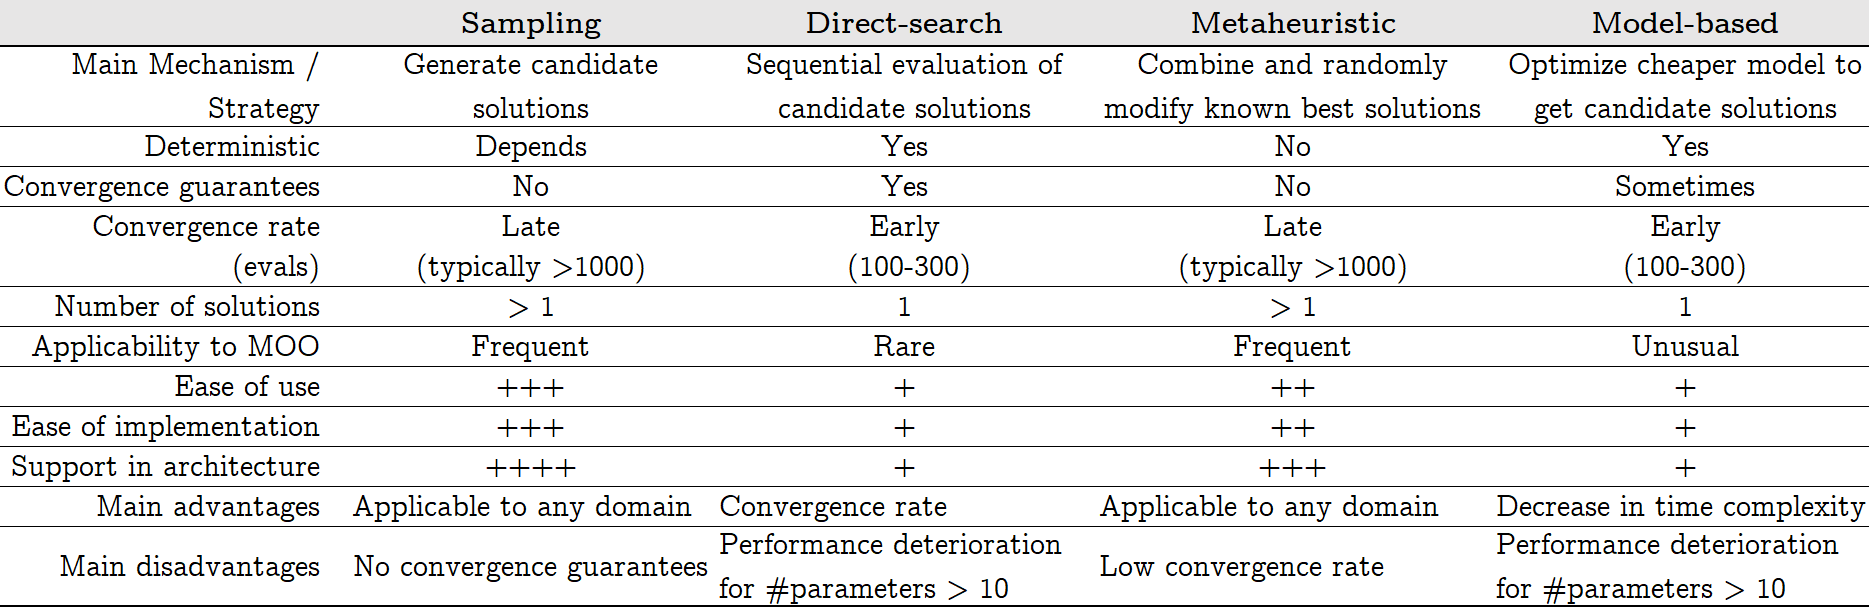
\includegraphics[width=1\textwidth]{tables_and_code/algorithms_comparison.PNG}
		\label{table:compare-dfo-algos}	
	\end{table}
	Conversely, direct-search and model-based algorithms are more difficult to use, implement, and less flexible, which represents a limitation towards their application in architectural domains. Moreover, the lack of ready-to-use tools involving algorithms from these categories is also limiting their application in architectural contexts. In fact, the existing non-metaheuristic tools are usually available as programming libraries, instead of being integrated in popular \ac{AD} tools. As a result, to use the optimization algorithms, architects often need some programming knowledge to integrate them. However, since architects typically lack this knowledge, they tend to opt for ready-to-use tools. Given this, it is not surprising that most of the existing building design optimization literature focuses on the application of algorithms from the metaheuristics category \cite{Evins2013,Nguyen2014,Hamdy2016}. 

	% Because of the distinct nature of architectural design problems, the arguments applied in architecture are not necessarily applicable to other fields, like science and engineering. 
	% In an attempt to exploit this fact, \ac{BPO} practitioners should dedicate a small amount of their total time budget to test various algorithms and different setup parameters, before finally settling for an optimization algorithm~\cite{Hamdy2016}.	

	However, in the light of the \ac{NFLT}, the need for more efficient optimization approaches fostered the development of tools providing algorithms with different properties. Particularly, plug-ins like Goat and Opossum enable the usage of algorithms from both direct-search and model-based classes. These tools offer optimization algorithms from the NLopt and RBFOpt frameworks, respectively, providing friendly, ready-to-use interfaces within Grasshopper, a visual programming environment that enables the parametric generation and performance evaluation of building designs for different values of the parameters. Comparisons between the algorithms existing in Goat and Opossum and the ones available in other metaheuristic optimization tools (e.g., Galapagos) have shown that, in general, direct-search and model-based algorithms seem to be more effective than metaheuristics in early stages of the optimization process \cite{Wortmann2017,Wortmann2017GABESTCHOICE}. More recently, some metaheuristics algorithms have been shown to perform consistently well in some optimization problems \cite{Waibel2018}. One can explore these performance fluctuations to find the most effective optimization algorithm for a specific problem. Indeed, several authors suggest that the selection of the optimization algorithm should be based on the results of several tests with different methods for a fixed number of evaluations or a fixed amount of time\cite{Hamdy2016, Wortmann2016BBO}. 
	
	%\todo{Transição brusca}
	%Optimization is a useful tool to address both single and multi-objective problems. In architecture, most optimization applications focus on single-objective problems and cover the three different derivative-free algorithms classes. However, the same does not happen with multi-objective problems, with only one of the classes being extensively applied to \ac{MOO} building design: the metaheuristics~\cite{Hamdy2016}. The main reason behind metaheuristics popularity is their broader adaptability to both varying degrees of complexity and to different problem domains~\cite{BlumRoli2003Metaheuristics}.
	
	Recent developments in multiple surrogate-assisted \acp{MOEA} in the fields of science and engineering made it possible to decrease the number of expensive evaluations in \ac{MOO} problems \cite{Hussein2016,Zapotecas-Martinez2016}. Generally, these techniques combine metaheuristics methods, which find more than one solution within a single execution, with surrogate models, which approximate the original objective functions. \cite{Diaz-Manriquez2016} provide a comprehensive overview of surrogate-assisted techniques for \ac{MOO} from the engineering perspective. 
	
	Given the wide variety of optimization algorithms, in order to select the most suitable algorithm for a specific optimization problem, it becomes necessary to measure their performance. In the next section, we discuss how to quantitatively compare the performance of optimization algorithms.
	
	%\todo{The relevance of these algorithms for design optimization is evident and translates into the multiplicity of studies that use them to optimize building designs' manifold aspects, including, among others, structural, lighting, thermal, energy consumption, and carbon-emissions \cite{Evins2011,Evins2012MOO, Wortmann2015AdvSBO,Wortmann2016BBO,Waibel2018}.}
	
	\subsection{Performance Indicators}
	\label{ssec:performance}
	Despite the large interest in \ac{MOO}, the question of how to quantitatively compare the performance of different algorithms still remains unanswered. Firstly, in multi-objective problems, the number of objectives is greater than in single-objective problems: the former considers a collection of vectors representing the Pareto-optimal solutions, whereas the latter considers scalar values. Secondly, it is often the case that the application of exact methods to \ac{MOO} contexts is impracticable due to the complexity introduced by underlying applications (e.g., simulation tools, physical experiments). In these cases, the generation of the true Pareto-optimal set requires vast computational resources and is often infeasible. Thirdly, despite the availability of alternatives to exact methods, such as metaheuristics algorithms (e.g., \ac{EA}, \ac{PSO}), these are not guaranteed to identify optimal trade-offs, instead yielding good approximations~\cite{Zitzler2003Metrics}. Finally, we are interested in knowing which of the non-exact algorithms yields better approximations for a given problem, hence prompting the need for assessing the performance of \acp{MOOA}.
	
	The notion of performance includes not only the quality of the results, but also the computational resources needed to generate such results. While the latter aspect is usually identical for both \ac{SOO} and \ac{MOO}, which either typically considers the number of expensive evaluations or the overall run-time on a particular computer, the quality aspect is considerably different. Because \acp{SOO} consider scalar valued objective spaces, the quality is defined in terms of the objective function: the smaller (or larger, in a maximization problem) the value, the better the solution. However, since \acp{MOOA} consider vector valued objective spaces, these require other concepts to measure solutions' quality, such as the Pareto dominance. Unfortunately, when considering the Pareto dominance concept, a few issues may arise, namely (1) the possibility of two solutions being incomparable, e.g., when neither dominates the other, or (2) having solutions in one set that either dominate or are incomparable to those in the other set of solutions, and vice versa. 
	
	Literature review evidences the existing struggle to define the meaning of quality with respect to approximation of Pareto-optimal sets~\cite{Knowles2002Metrics,Riquelme2015}. However, the quality of Pareto sets is usually evaluated in terms of three aspects: (1) cardinality, meaning larger sets of solutions, (2) diversity, meaning that solutions should be as uniformly distributed as possible, so as to obtain a representative set of solutions covering to larger extents the different trade-offs, and (3) accuracy, meaning that solutions should be as close as possible to the true Pareto-optimal set or Pareto Front. 
	
	For the past decades, several indicators have been proposed to measure the quality of Pareto sets with respect to three aspects: cardinality, diversity, and accuracy. This dissertation considers a representative set of indicators to measure the quality of \acp{MOOA}' results, ranging from unary to binary quality indicators. The former assign to each approximation set a number that reflects a certain quality aspect, whereas the latter assign numbers to pairs of approximation sets. In the following sections, we discuss some of the considered indicators. The term \textit{approximation set} is used to denote the Pareto Front returned by an optimization algorithm, and the term \textit{reference set} is used to denote the true Pareto Front or, whenever that is not possible, an estimate of the true Pareto front. 	
	
	% ---------------------------
	% Unary Indicators 
	% ---------------------------
	\subsubsection{Unary Indicators}
	%% https://github.com/PastelBelem8/MscThesis/blob/metrics/src/indicators/MOOIndicators.jl
	% Cardinality 
	With regards to the cardinality aspect, there are essentially three indicators \cite{Veldhuizen1999GD}:
	\begin{itemize}
		\item \textbf{\ac{ONVG}} computes the number of nondominated solutions in the approximation set. Similarly, \textbf{\ac{ONVGR}} computes the ratio of these optimal solutions with regards to a reference set.
		% ER
		\item \textbf{\ac{ER}} computes the proportion of false-positives in the approximation set, i.e., the ratio of optimal solutions in the approximation set that are not optimal in a given reference set. Lower values of \ac{ER}, represent better approximation sets. 		
	\end{itemize}
	
	The first cardinality indicator is based on the intuition that a good approximation set would have many optimal solutions. However, this indicator alone does not suffice to provide an accurate measure, as it privileges quantity over quality of solutions, i.e., it often qualifies approximation sets having dozens or hundreds of dominated solutions as being better than sets that provide fewer nondominated solutions. This completely distorts the initial idea of finding the best set of nondominated solutions, i.e., Pareto front. On the other hand, \ac{ER} focuses on errors instead of focusing on optimal solutions. As a result, it penalizes larger approximation sets that, despite having a more representative set of the real optimal solutions, have made more errors than other approximation sets with fewer solutions and, potentially, less errors. 
	
	% || Diversity / Distribution ||
	To complement cardinality indicators, it is often advisable to consider the diversity aspect of approximation sets as well. Two well-known diversity-based indicators are\cite{Zitzler2003Metrics}:
	\begin{itemize}
		\item \textbf{Spacing} (or Set Spacing) \cite{Schott1995} computes the variance of the Manhattan distances\footnote{Manhattan distance is obtained by computing the absolute values of the difference between solutions.} between each nondominated solution and its closest neighbor. It measures how well-spaced the solutions from the approximation set are. A value of zero represents equally spaced nondominated solutions. 
		\item \textbf{Maximum Spread} (or \textbf{$M_3^\ast$}) \cite{Zitzler1999} computes the Euclidean distance between the bounds of each objective dimension. It measures the extent of the objective space in each dimension by calculating the distance between the maximum and minimum of each objective. A greater value indicates larger coverage of the objective space.
		
		%\item \textbf{Entropy} uses Shannon's entropy~\cite{Shannon1948} concept to measure the uniformity of the approximation set distribution. This indicator makes the assumption that each solution provides some information about its vicinities, thus modeling each solution with Gaussian distributions. These distributions add up to form a density function capable of identifying peaks and valleys in the objective space, corresponding to dense and sparse zones, respectively. 
		
		%\item \textbf{Diversity Metric} is similar to the Entropy indicator. However, it projects the solutions of both the approximation set and the reference set to a hyperplane which is subdivided uniformly. It assigns each interval two numbers: one number marking whether that interval contains at least one optimal solution in the reference set, and the second number marking whether the interval in addition to the optimal solution in the reference set, also contained at least one solution in the approximation set. Then, the diversity measure is the sum of the score of each interval, which are assigned using a sliding window technique (considering one interval and its immediate neighbors) based on the value of the marks\footnote{The scoring function considers the distribution of the marks in three consecutive grids.}. So, the diversity of the reference set considers the value of the first marks, whereas the diversity of the approximation set considers the values of the second marks. In the end, the diversity metric is given by the relative difference between the diversity of the approximation set and the diversity of the reference set. The best diversity possible is achieved if all intervals enclose at least one point\cite{Deb2002DM}.
		% Then, it computes the ratio between the number of intervals that have at least one nondominated solution from both sets and the number of intervals that have at least one nondominated solution of the reference set. Higher values of the diversity metric imply a better distribution and higher diversity of the approximation set when compared to the reference set itself. 
		
	\end{itemize}
	
	While these indicators are more robust, alone, they will not necessarily identify sets having Pareto optimal solutions, as they prioritize sets where solutions are spaced evenly apart or cover broader regions of the objective space~\cite{Veldhuizen1999GD}. Moreover, because most of them assume that the Pareto front will be continuous, they may behave erroneously when facing problems with disconnected Pareto fronts. %The diversity metric attempts to alleviate these limitations by comparing the nondominated solutions of the approximation set with those of the reference set \cite{Deb2002DM}.
	
	% || Accuracy ||
	The previous metrics are not good indicators of how close the approximation sets really are to the reference set. To obtain a measure of the convergence of the results, one should consider accuracy indicators, such as~\cite{Veldhuizen1999GD}:
	\begin{itemize}
		% MPFE
		\item \textbf{\ac{MPFE}} computes, for each solution in the approximation set, the minimum Euclidean distance to the closest solution in a given reference set, returning the maximum of those distances. In other words, it returns the maximum error of the approximated Pareto Front. Lower values of \ac{MPFE} imply better approximation sets. 
		% Generational Distance
		\item \textbf{\ac{GD}} computes the average distance of an approximation set to a given reference set by computing the distance of the solutions in the approximation set to the nearest points in a given reference set averaged on the number of solutions in the approximation set. A value of $0$ indicates that all the solutions in the approximation set are in the reference set. Different authors\cite{Zitzler2000m1m3} refer to this metric as \textbf{$M_1^\ast$}.
	\end{itemize}
	
	Accuracy indicators, like the previous indicators, can also produce misleading results and, therefore, should be considered together with other metrics. In general, both indicators have flaws. On the one hand, \ac{MPFE} focuses on the maximum error of an optimal solution in the approximation set, when compared to the reference set. As a result, approximation sets, whose points are closer to the Pareto front but that have an outlier, will have higher values of \ac{MPFE} than other approximation sets, whose points are further away from the reference set but at a smaller distance than the outlier is from the reference set. On the other hand, \ac{GD} has also been shown to behave erroneously, especially due to its dependency on the cardinality of the approximation set ~\cite{Ishibuchi2005GDIGD}. The final set of indicators considers all aspects simultaneously \cite{Li2017Rmetrics}:
	\begin{itemize}
		% Hypervolume
		\item \textbf{\ac{HV}} (or Lebesgue measure or S-metric) measures the size of the objective space covered by an approximation set, i.e., it measures the volume of the dominated space. It provides the unique and desirable properties of (i) Pareto \textit{compliance}, i.e., an approximation set which completely dominates another, will necessarily have a greater volume than the latter, and (ii) convergence guarantees, i.e., any approximation set that achieves the maximum possible volume is guaranteed to contain all Pareto-optimal solutions.
		% Inverted GD
		\item \textbf{\ac{IGD}} is the opposite of \ac{GD}, instead computing the average distance between a given reference set and the approximation set. \ac{IGD} computes the distances between each solution in the reference set and its closest solution in the approximation front, averaged over the size of the reference set. When the solutions in the reference set are well distributed, smaller values of \ac{IGD} suggest better and well-distributed approximation sets. Previous works have referred to this metric as \textbf{$D1_R$}.%\todo{Save REFs, a verdadeira ref está no Hansen1998}. 
	\end{itemize}
	
	Despite considering the diversity and accuracy of Pareto fronts, \ac{IGD} is still Pareto non\nobreakdash-\hspace{0pt}compliant and has been shown to behave erroneously under certain conditions. Conversely, \ac{HV} is the only metric that exhibits the Pareto-compliance property. However, its usage is often impractical in problems where the number of objectives is greater than ten, due to its exponential growth with the number of objectives \cite{Ishibuchi2005GDIGD}.
	
	\subsubsection{Binary Indicators}
	In situations where the original Pareto-optimal set is not available, binary indicators provide a way to compare approximation sets. Among the most frequently used indicators, we emphasize \cite{Zitzler2003Metrics,Li2017Rmetrics}:
	\begin{itemize}
		% \item \textbf{Two set coverage} (or $C$) yields the number of solutions in one approximation set that are dominated by at least one of the solutions of the other approximation set. A value of $1$ suggests that the second approximation set is completely dominated by some solutions in the first one, whereas a value of $0$ represents the situation when none of the solutions of the second approximation set is covered by the first approximation set.
		
		\item \textbf{Epsilon Indicators} ($\epsilon$) give a factor by which an approximation set is worse than another considering all objectives, i.e., given two sets $A$ and $B$, it computes the smallest amount $\epsilon$ by which $A$ must be translated, so that every solution in $B$ is dominated by at least one solution in $A$.
		
		\item \textbf{R-metrics} consider a family of indicators where the quality of each approximation set is defined according to a set of utility functions, and the larger the utility value of some set, the better the quality. R-metrics declare that the best approximation set will be the one that is better with regard to most utility functions:
		\begin{itemize}
			\item \textbf{$R1$} determines whether an approximation set is better, equal, or worse than other. 
			\item \textbf{$R2$} computes the expected mean difference in the utilities of both approximation sets.
			\item \textbf{$R3$} computes the expected mean relative difference in the utilities of both approximation sets.
		\end{itemize}
	\end{itemize}

	Although binary indicators are useful for comparing different approximation sets and their relations. While the former particularizes these relations to be defined as the relative difference among two approximation sets, the latter incorporates utility functions predefined by users to introduce preferences over the different objectives and, consequently, to influence the quality of each set. 
	
	% When comparing the usefulness of binary indicators, these usually aim at comparing different approximation sets and not necessarily the quality of the sets. This is the case of the two set coverage indicator, which allows to compare the existing Pareto-dominance relation between two sets, but does not allow to infer any other information (e.g., how worse one set is regarding the other). Moreover, this indicator becomes erroneous when the two sets are incomparable, i.e., neither dominates the other~\cite{Zitzler2003Metrics}. In contrast to the two set coverage indicator, the epsilon family indicators enable more informed comparison among two different approximation sets, as it provides a measure of the relative difference between the two sets. Finally, because the R-metrics incorporate utility functions, the user is able to introduce a preference over the objectives, thus influencing the optimality of each set. 
	
	\section{Optimization in Architecture}	
	\label{sec:optimizationtools}
	
	For years, multiple derivative-free optimization libraries have been developed (e.g., NLopt, RBOpt, Platypus, jMetal, and MOEAFramework). However, in order to use them within architectural practices, architects had to code integration scripts to connect the simulation-based evaluation of the different parametric models with optimization libraries. Moreover, these libraries often lack post-processing and visual features, which antagonizes the readability and comprehension of the results~\cite{Attia2013,Nguyen2014}.
	
	Several plug-ins have been developed in an attempt to reduce the limitations associated to the coupling of simulation tools and mathematical optimization frameworks, thus providing a seamless connection between the 3D models produced in computational design tools, the analytical models, and the optimization frameworks. Given the visual nature of architectural projects, these plug-ins provide friendly, ready-to-use optimization interfaces, which are usually coupled to a few post-processing and visual features to enhance the intelligibility of optimization results. 
	
	Currently, existing optimization plug-ins are implemented on top of visual algorithmic tools, like Grasshopper and Dynamo. Amongst \ac{BPO} practitioners, the most relevant optimization plug-ins are Galapagos, Goat, Octopus, Opossum, and Silvereye, which are all implemented on top of Grasshopper. Even though Dynamo supports an optimization plug-in, Optimo, this is less used in practice and, therefore, will not be discussed in this dissertation. In the following sections, we briefly discuss Grasshopper's optimization plug-ins. 
	
	% Begin Optimization Plug-ins Figure -------------------------------------------------------
	%\begin{figure}
	%	\centering
	%	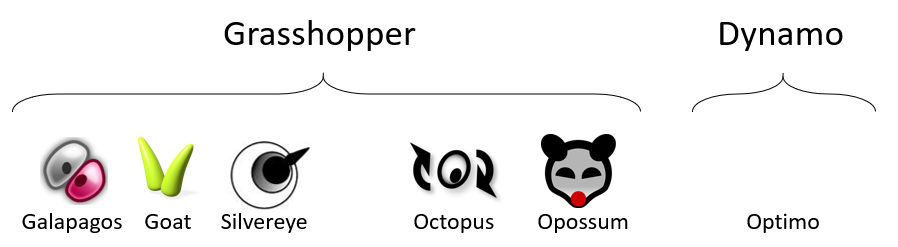
\includegraphics[width=\textwidth]{Images/Background/opt-plugins.PNG}
	%		\caption[Optimization Frameworks in the Architectural Practice]{Optimization frameworks currently used in architectural practices.}
	%	\label{fig:opt-plugins}
	%\end{figure}
	% End Figure -------------------------------------------------------
	
	\subsection{Galapagos}
	\label{subsec:galapagos}
	% General description of Galapagos, intuition
	Galapagos is a generic plug-in, implemented on top of Grasshopper, for the application of metaheuristics algorithms by non-programmers. 
	% Optimization Algorithms
	Particularly popular amongst architects for its \textit{\ac{GA}} implementation \cite{Wortmann2017ADO}, Galapagos also provides another global metaheuristic solver, called \textit{Simulated Annealing}. 
	
	% User Experience
	To use one of the solvers, architects must first define a program using Grasshopper's components, such as sliders, value lists, area, distance, among others, organized in three distinct parts: (1) the Input, where they specify the design parameters; (2) the Generation, where they create the design's algorithmic model that, when instantiated with the parameters' values, generates the 3D model; and (3) the Analysis, where they define the analysis or objective function, which they seek to optimize. 
	
	After creating the program, the architect must drag the Galapagos' component, still within the Grasshopper environment, and connect it to the design parameters and to the objective function. Note, however, that Galapagos requires the variables, provided as inputs, to be defined in terms of slider components, interpreting their numerical range as the variables' lower and upper bounds, and the objective function to be outputted to a number component. The Galapagos' component refers to the variables as \textit{genome} and to the objective function as \textit{fitness}.
	
	Galapagos' \ac{GUI} is displayed upon double-clicking the Galapagos' component (see \cref{fig:galapagosoptions}). The interface is simple, friendly, intuitive, and well-organized. Moreover, all options are filled by default, thus promoting a ready-to-use (or click-and-run) interaction, which makes it easy to use by less experienced users. Unfortunately, more experienced users might feel frustrated using this plug-in, as they are only able to modify a few parameters of the solver (e.g., population size and number of maximum evaluations), thus lacking a finer control over the process. 
	
	In addition to not requiring any integration efforts or any programming-related knowledge to setup and use its capabilities, Galapagos also provides a visually rich experience, by providing different runtime graphical views of the optimization process. Galapagos supports different views depending on the optimization solver being used (see \cref{fig:galapagosviewsa} and \cref{fig:galapagosviewsb}):
	\begin{itemize}
		\item A fitness graph that either represents the distribution of fitness values in the population discriminated by generations. Exhibited for both solvers;
		\item A similarity representation graph that represents solutions that are similar to each other, and marks solutions that contribute to the creation of the next generation with black dots, whilst non-contributors are marked with a red cross. Exhibited for the \textit{\ac{GA}} solver;
		\item A vertical parallel coordinates graph, where each vertical line corresponds to a parameter, and solutions are represented as line segments connecting different parameters' values. Exhibited for the \textit{\ac{GA}} solver;
		\item A ranked list of the best solutions found. Exhibited for both solvers;
		\item A temperature graph, representing the temperature decrease rate of the \textit{Simulated Annealing} process with each time step. Exhibited for the \textit{Simulated Annealing} solver.
	\end{itemize}
	
	Overall, these views provide visual feedback about the course of the optimization run and highlight the best solutions found up to that generation. In the end, the user is able to navigate through generations and re-instantiate these solutions in the corresponding \ac{CAD} tool, and, consequently, better understand the obtained results. Moreover, the ranked list of results allows the user to select the one he prefers the most amongst multiple optimal solutions found by the solver. Unfortunately, Galapagos lacks logging mechanisms, which causes the information about the optimization, that is enclosed within these views, to be lost as soon as the \ac{GUI} is closed. 
	\begin{figure*}[]
		\centering
		\subfigure[]{%
			\label{fig:galapagosoptions}%
			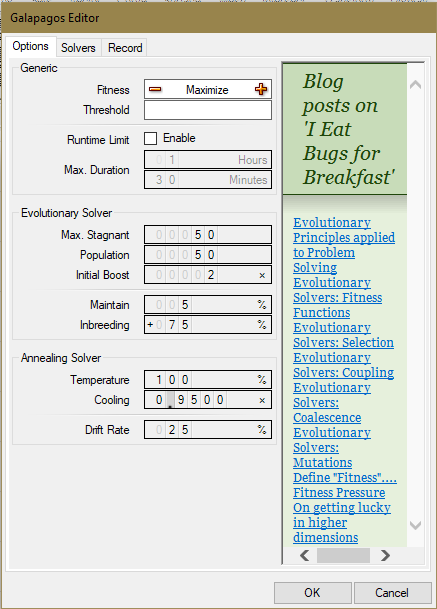
\includegraphics[width=0.30\textwidth]{Images/Background/Galapagos/Galapagos-algorithms-setup.PNG}}%
		\hfill
		\subfigure[]{%
			\label{fig:galapagosviewsa}%
			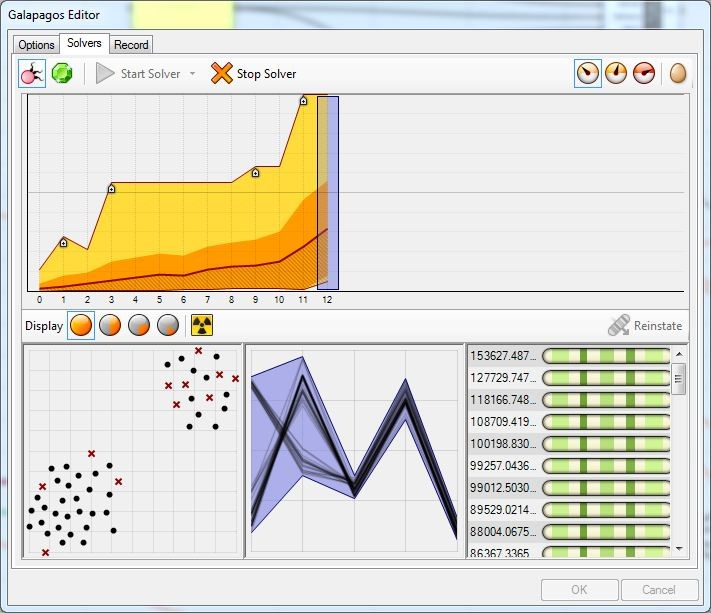
\includegraphics[width=0.345\textwidth]{Images/Background/Galapagos/galapagosvis.JPG}}%
		\hfill
		\subfigure[]{%
			\label{fig:galapagosviewsb}%
			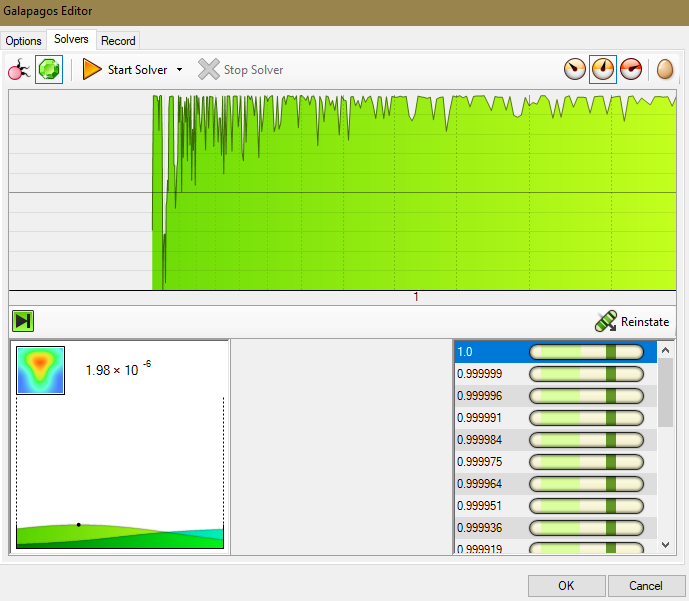
\includegraphics[width=0.345\textwidth]{Images/Background/Galapagos/galapagos-sa-results-2.PNG}}%
		
		\caption[Galapagos GUI]{Three views of the Galapagos' \ac{GUI}: (a) Solver's configuration menu (b) Graphical views for the \textit{\ac{GA}} solver (c) Graphical views for the \textit{Simulated Annealing} solver}
		\label{fig:galapagos}
	\end{figure*}
	
	% ----------------- [GOAT] ------------------
	\subsection{Goat}
	% General description, intuition
	Goat is a generic optimization plug-in, implemented on top of Grasshopper, designed to enable non\nobreakdash-\hspace{0pt}programmers to solve numerous problems.
	Unlike Galapagos, Goat interfaces the NLopt mathematical optimization library to provide single-objective algorithms from all the derivative-free classes mentioned earlier, including one global direct-search (\textit{\ac{DIRECT}}), one local direct-search (\textit{SUBPLEX}), one global metaheuristic (\textit{CRS2}), and two local model-based algorithms (\textit{\ac{COBYLA}} and \textit{\ac{BOBYQA}}). 
	
	Goat is strongly influenced by Galapagos, also requiring a user program in Grasshopper containing the definition of the problem. The user drags the Goat's component to the program, connecting it to the design parameters and the objective function, which, like Galapagos, must be provided as sliders and number components, respectively.
	
	Goat's \ac{GUI} is displayed after double-clicking the Goat's component. This interface comprises a single menu, which is simple and straightforward to use. Like Galapagos, Goat is distributed in a ready-to-use format with all the extra configuration values filled by default. As a result, non-expert programmers can easily explore this tool to address complex problems. Unfortunately, Goat provides no options for a more experienced user to configure the algorithms, except to configure the initial point of the search.
	
	Despite requiring no additional efforts to use Goat's optimization capabilities, the absence of visual and interactive mechanisms severely hinders Goat's reputation. Firstly, it provides no visual feedback (e.g., solution lists, plots) about the course of the optimization run. Secondly, it also does not create log files to monitor the optimization process. Thirdly, the user is not able to interact with the optimization process. Finally, it returns a single optimal solution, whose values are represented in the sliders and number components. All these reasons contribute to a non-informed and non-traceable optimization process that inspires little confidence in the obtained results. 
	
	% Begin Goat-Options Figure -------------------------------------------------------
%	\begin{figure}
%		\centering
%		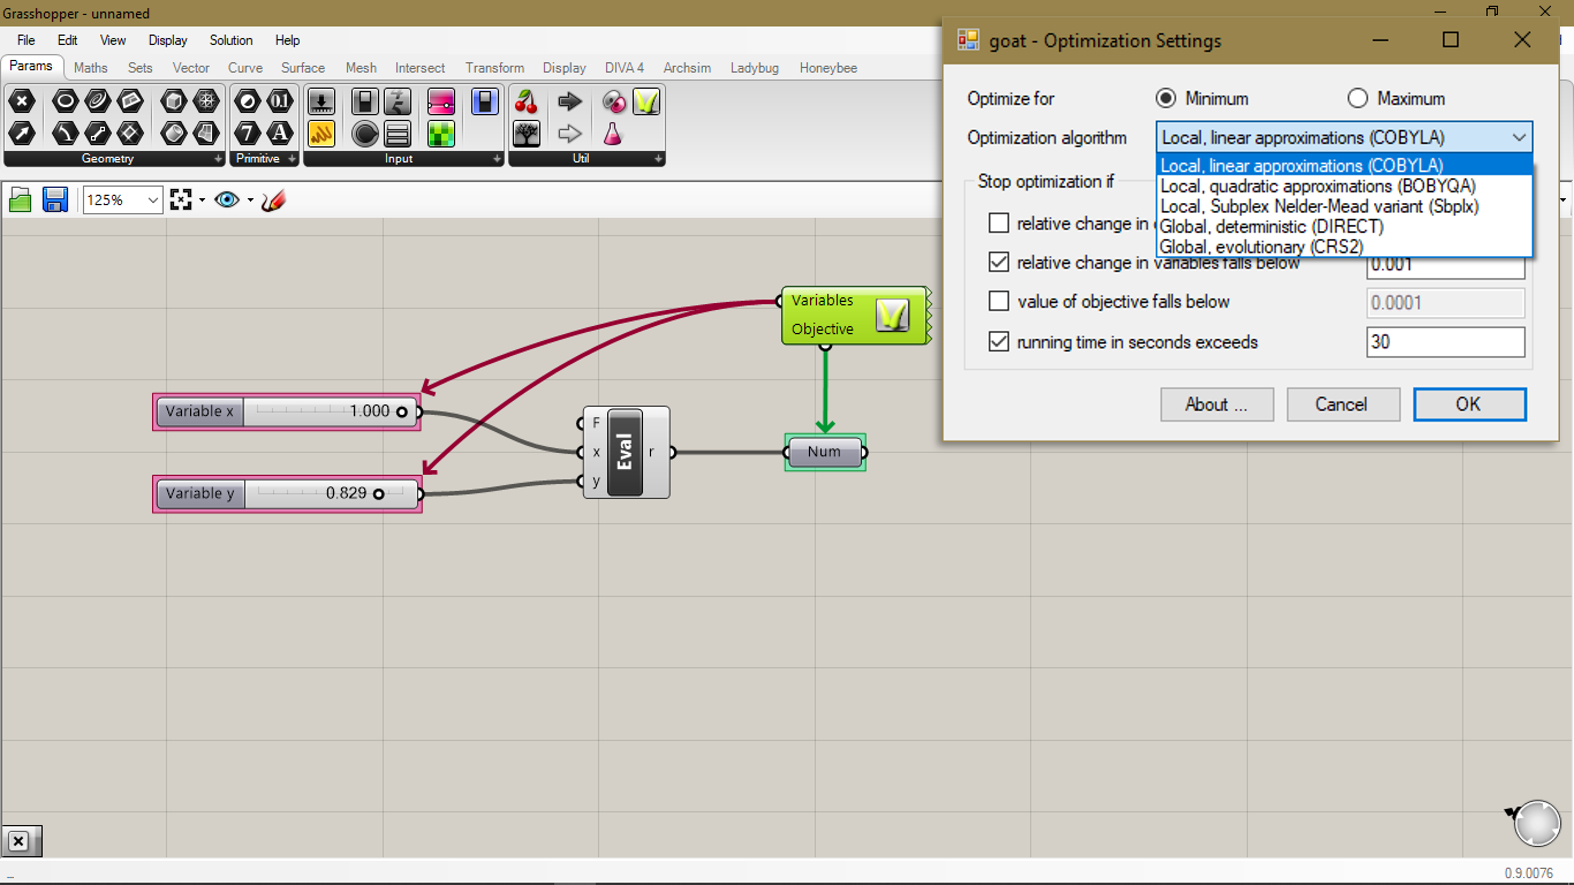
\includegraphics[width=1\textwidth]{Images/Background/Goat/general-view.png}
%		\caption[Goat GUI]{Simple view of the Grasshopper's script with the problem definition and the Goat component. The curves on the left (pink) link to the variables and the one on the right (green) links to the objective, On the foreground, the \ac{GUI} exhibits the list of available algorithms within Goat.}
%		\label{fig:goat}
%	\end{figure}
	% End Figure -------------------------------------------------------	
	
	
	% ----------------- [SILVEREYE] ------------------
	\subsection{Silvereye}
	Silvereye is a generic optimization plug-in, implemented on top of Grasshopper, developed under the same design principles as Galapagos to enable non-experts to solve complex optimization problems. Unlike Goat which interfaces with a well-known optimization library, Silvereye exposes C\# implementation of a global single-objective \ac{PSO} algorithm, as described in \cite{Cichocka2017SILVEREYE}. 
	
	Similarly to the previous tools, Silvereye also requires the definition of the problem in Grasshopper, and that the variables and the objective function are represented by sliders and number components, respectively. Thus, it does not require any additional effort in order to be used.
	
	Like Galapagos, the user must double-click Silvereye's component in Grasshopper to visualize its \ac{GUI}. Besides being very simple and intuitive to use, Silvereye also allows less experienced users to start using the tool immediately by providing default values to the extra configuration parameters. As users gain more experience, they might decide to change some configurations associated with the solver. One other difference to Galapagos is the ability to save the solver's configurations so that it can be used in subsequent runs.
	
	Regarding its visual capabilities, Silvereye resembles Goat, providing no graphical views of the optimization run's state. However, Silvereye does present a list that is updated in real-time with the value of the best fitness value per iteration, which can be exported to a file and then used to create fitness graphs. Unfortunately, since this file merely contains the fitness values, the user is not able to trace them back to the values of the design parameters which originated them. Moreover, despite the existence of a functionality in the first menu to create a log file, this file only contains information about the temporal behavior of each evaluation. While this information is useful to monitor and identify irregularities during the optimization run, it does not provide enough information to traceback the error. 
	
	Overall, the lack of visual feedback in the form of graphs hinders the comprehension and confidence on the results. The ranked list helps filling this gap, as long as there are multiple solutions and the user is able to visualize them in a \ac{CAD} tool.
	
%	\begin{figure*}[htbp]
%		\centering
%		\subfigure[]{%
%			\label{fig:silvereye1}%
%			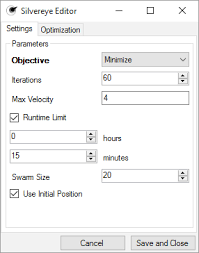
\includegraphics[width=0.40\textwidth]{Images/Background/Silvereye/silvereye.png}}%
%		\hfill
%		\subfigure[]{%
%			\label{fig:silvereye2}%
%			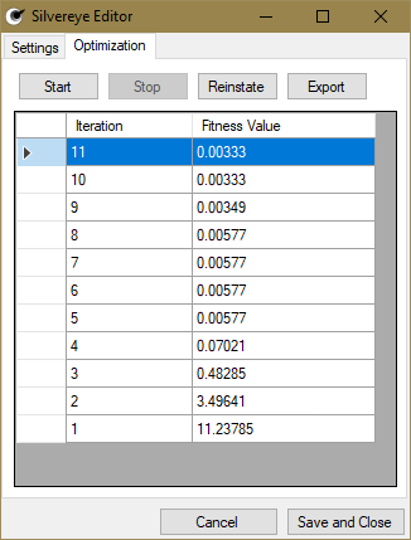
\includegraphics[width=0.40\textwidth]{Images/Background/Silvereye/silvereye2.png}}%
%		
%		\caption[Silvereye GUI]{Two views of Silvereye's \ac{GUI}: (a) Solvers configuration menu (b) Optimization control and results menu}
%		\label{fig:silvereye}
%	\end{figure*}
	
	%------------------ OPOSSUM ----------------------
	\subsection{Opossum}
	Opossum (OPtimizatiOn Solver with SUrrogate Models) is a generic plug-in, developed on top of Grasshopper, that explores Galapagos' ideas to confer non-programmers an easy way to tackle a wide variety of optimization problems. Opossum interfaces with the model-based RBFOpt library, presenting two single-objective variants of the global \ac{RBF} algorithm. 
	
	In terms of usability, Opossum also resembles Galapagos, only requiring the definition of the problem in a Grasshopper program. To use the Opossum's solvers, the user must drag the Opossum's component to the Grasshopper program and connect it with the variables and the objective function components.
	
	Opossum's \ac{GUI} is simple, friendly, intuitive, and well-organized, depicted in \cref{fig:opossum}. In contrast to other plug-ins, Opossum presents different menus tailored for different levels of expertise. On the one hand, Opossum promotes a ready-to-use format, in order to ensure that less experienced users are able to use Opossum's capabilities. Therefore, Opossum provides two top-level configurations menus for which the values are already filled by default. On the other hand, Opossum also provides more experienced users with the ability to create a finer configuration for the optimization solvers and, thus, achieve potentially more efficient optimization processes. 
	
	% Begin Opossum-Options Figure -------------------------------------------------------
	\begin{figure}
		\centering
		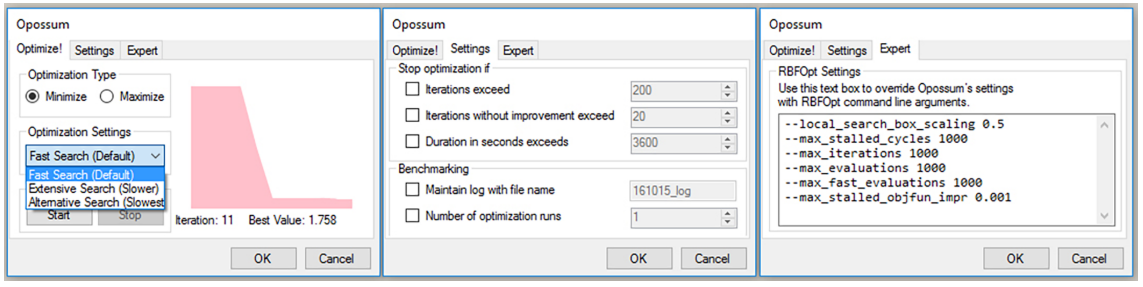
\includegraphics[width=1\textwidth]{Images/Background/Opossum/opossum_1.png}
		\caption[Opossum GUI]{The three views of Opossum's \ac{GUI}. Image retrieved from~\cite{Wortmann2017Opossum}}
		\label{fig:opossum}
	\end{figure}
	% End Figure -------------------------------------------------------
	
	The main drawback of this plug-in lies in its visualization features. Although Opossum presents a fitness graph (see \cref{fig:opossum}) that is very useful for obtaining immediate feedback about the course of optimization, it does not provide an overview of the extent of the design space that is being explored, nor about the distribution of the designs that are being evaluated. Moreover, Opossum supports the creation of a log file that records all the solutions evaluated during the optimization run. Using other post-processing tools, the user can either produce more insightful visualizations of the data, or re-use this information to create more accurate surrogate models, for example, for sensitivity analysis.
	
	One other disadvantage of this plug-in is the fact that the result of the optimization run is a single solution, instead of multiple ones. As a result, the intelligibility of results and the confidence on the process is greatly hindered, especially due to its low visual support. 
	
	% ------------- [ Octopus ] -----------------
	\subsection{Octopus}
	
	Octopus is a generic plug-in, developed on top of Grasshopper, that allows non-programmers to address a wide variety of \ac{MOO} problems. Octopus exposes two global metaheuristics algorithms to search for Pareto-optimal solutions: \textit{\ac{SPEA2}} and \textit{Hypervolume Estimation algorithm} (\textit{HypE}). These algorithms have been reported to yield promising results on numerous \ac{MOO} test problems~\cite{Zitzler2001SPEA2,Zitzler2011HypE}. 
	
	Even though Octopus was originally designed exclusively for optimization purposes, more recently, its focus has grown to include other \ac{ML} utilities, like supervised and clustering mechanisms. In fact, whereas previous Galapagos-based plug-ins focused exclusively on optimization, Octopus covers multiple functionalities implemented as Grasshopper components.
	
	The second difference affects the user program. Like Galapagos, Octopus require the definition of the problem's variables and objective functions. However, since Octopus focuses on \ac{MOO}, the user has to ensure that all the results of the objective functions are aggregated in a single number component and then connected to the Octopus component. Additionally, because Octopus only performs minimization, the problem definition must be modified to guarantee that all objectives are being minimized. One other important difference is that Octopus is able to tackle constrained problems. In this case, the hard constraints must be represented by a boolean component, and then connected to the Octopus component.
	
	%After creating the Grasshopper script, Octopus \ac{GUI} can be accessed by double-clicking the Octopus component (see \cref{fig:octopus2}). 
	Despite its simplicity and friendliness, Octopus \ac{GUI} (see \cref{fig:octopus}) is poorly organized and overloaded with information, hence making it difficult for a non-experienced user. Although Octopus is distributed in a ready-to-use format, this plug-in presents mechanisms to fine-tune a few parameters of the solvers. Even more surprising is the ability to change some of these parameters (e.g., elitism, mutation probability, crossover rate, mutation type) during runtime, thus allowing the user to influence the optimization process.
	
	Octopus provides good support in terms of graphical feedback, providing three distinct views of the optimization problem (see views 1, 8, and 10 in \cref{fig:octopus}), namely:
	\begin{itemize}
		\item Solutions' objective space graph, which illustrates the distribution in the objective space of the solutions obtained during the optimization run. This graph also exhibits the approximated Pareto front that is currently known by the algorithm;
		\item Horizontal parallel coordinates graph, which serves the same purpose of the vertical parallel coordinates graph and that provides a view over the different design solutions that have been tested;
		\item Objective convergence graphs (one for each objective), showing the upper- and lower-bounds of the Pareto front (dark gray) and the elite (light gray) of the number of history generations.
	\end{itemize} 
	
	Octopus is capable of solving problems with up to five objective dimensions, using the three spatial dimensions, color, and size to represent them. However, the readability of these graphs becomes difficult with more than three dimensions. In addition to the strong visual mechanisms, Octopus provides mechanisms to interact and instantiate each solution in the corresponding \ac{CAD} tool, which not only gives confidence about the results, but also allows the user to better understand them. Optionally, Octopus makes it possible to disable the real-time visualization of the optimization process with the aim of reducing the associated overhead.
	
	One other important feature of Octopus is the ability to create logs with the information about the evaluated solutions discriminated by generation. The only setback is that it does not allow the create of a single file simultaneously containing the information about the design parameters and the objectives. 
	
	\begin{figure}[h]
		\centering
		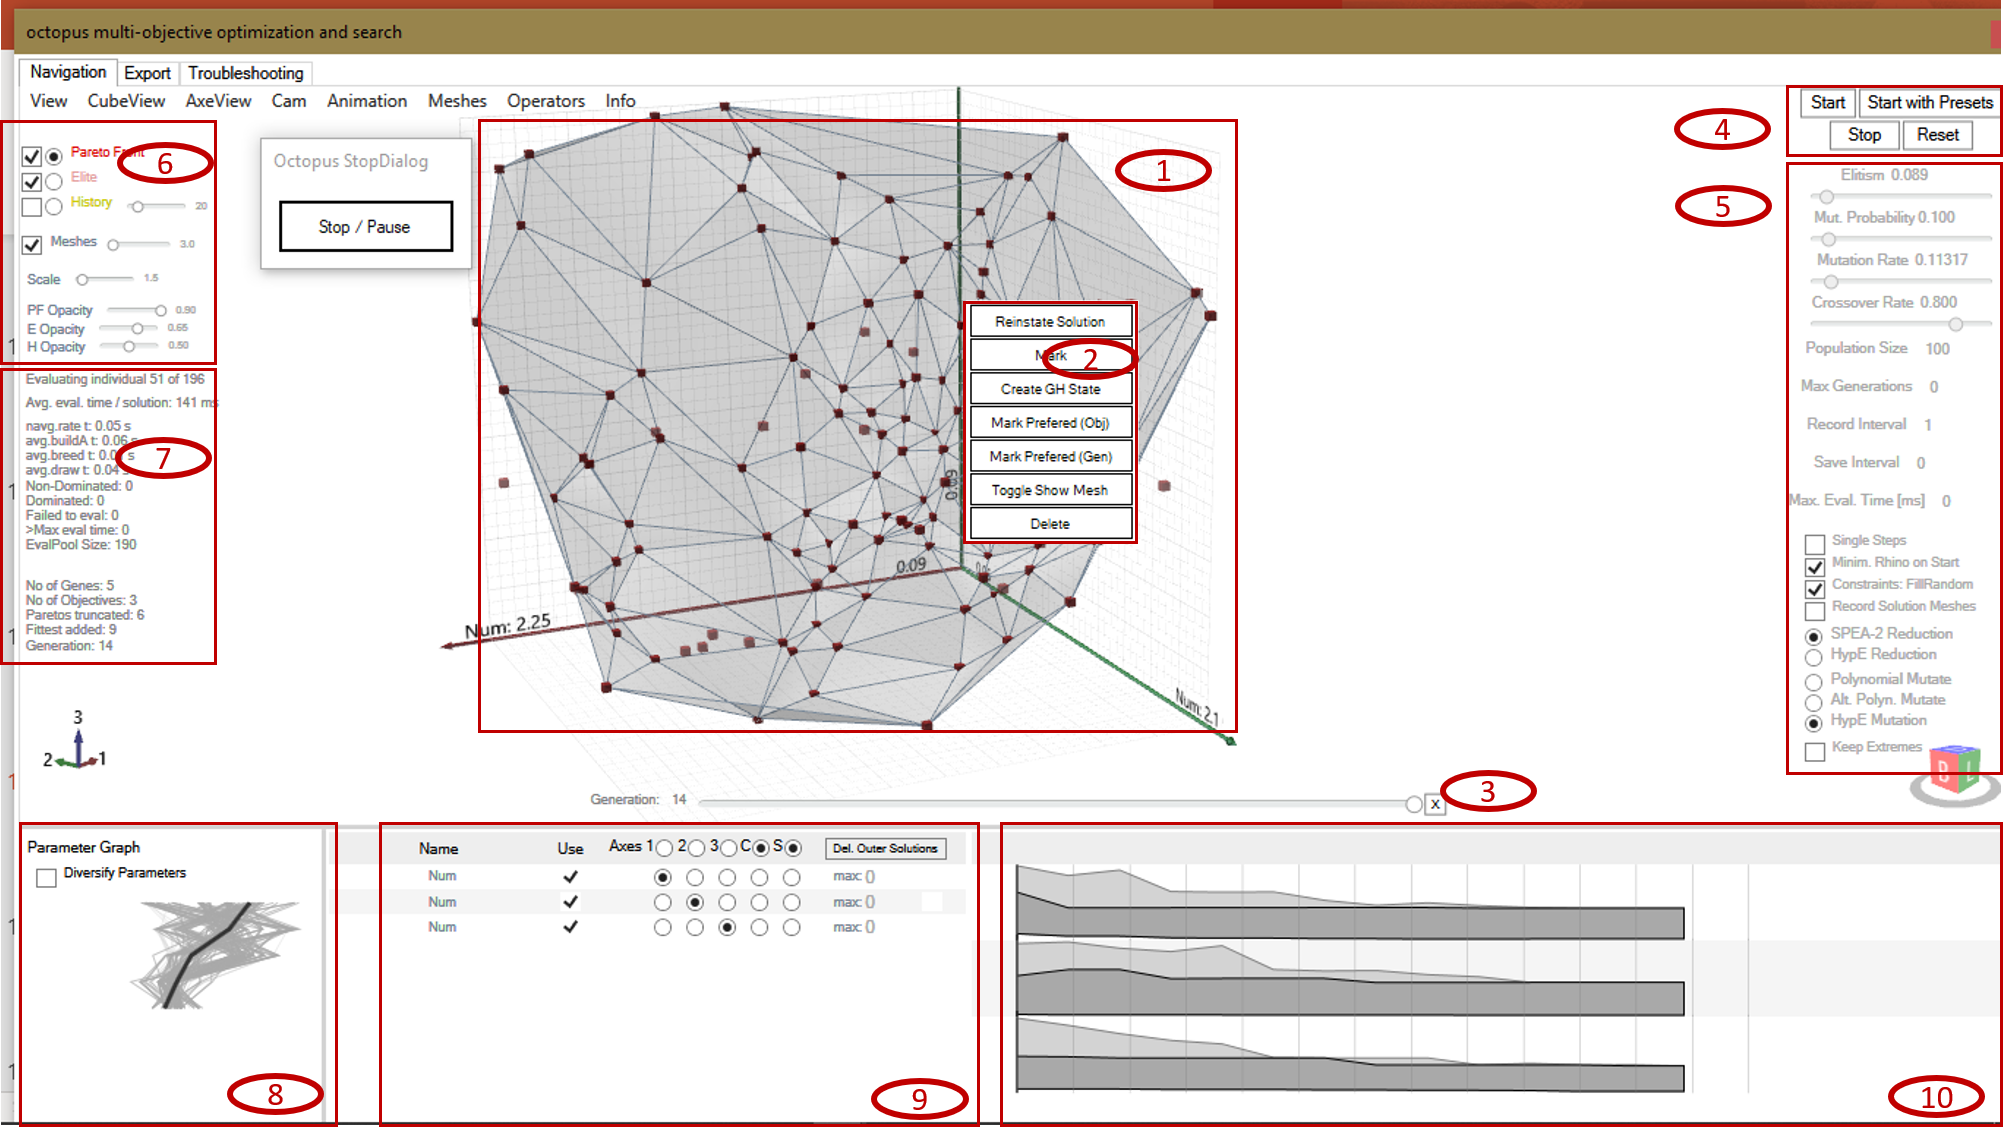
\includegraphics[width=1\textwidth]{Images/Background/Octopus/octopus-menu.png}
		\caption[Octopus GUI]{Octopus's \ac{GUI}: (1) Solutions' Objective Space, (2) Solution's context menu, (3) Generation's history slider, (4) Process control options, (5) Algorithm Settings, (6) Display Settings, (7) Statistics, (8) Parallel Coordinates Graph, (9) List of Objectives (10) Convergence graphs per Objective}
		\label{fig:octopus}
	\end{figure}
	
	
	% ------- ------- [OPTIMO] -------- ----------
%	\subsection{Optimo}
%	\label{subsec:Optimo}
%	
%	Optimo \cite{OPTIMO} is a generic plug-in, implemented on top of Dynamo, that allows non-programmers to address a wide variety of \ac{MOO} problems in the context of a \ac{BIM} tool. 
%	
%	Optimo interfaces the \ac{MOO} metaheuristics library, jMetal.NET, and its current version merely supports the \ac{NSGA-II} algorithm\cite{Deb2002}.
%	
%	To use the solver, users must create the Dynamo program that encodes the problem definition, but also encode the optimization algorithm. To create the latter, Optimo provides four Dynamo nodes:
%	\begin{itemize}
%		\item Initial Solution list, which generates the initial set of random design configurations within a provided range and with the specified size of population;
%		\item Assignment of Fitness Function Results, which evaluates and assigns the objective values to each configuration; 
%		\item Generation Algorithm, which takes the parent population and generates the children population;
%		\item Sorting, which uses the Pareto Front sorting to sort the solutions
%	\end{itemize} 
%	
%	Compared to the previous plug-ins, Optimo demands larger initial investments for the production of the program. Whereas less experienced users might find it more difficult to use, more experienced ones might adjust the algorithm to their needs.%, which directly results from the finer-grain control of Optimo. 
%	In practice, instead of providing a default template, Optimo fosters the constant arrangement of the algorithm's nodes everytime a new optimization process is to be applied, which can quickly become monotonous and tiresome. Moreover, Optimo does not have a explicit \ac{GUI} editor, instead being directly integrated in the Dynamo environment in the form of nodes.
%	
%	% Visual
%	Regarding the visual mechanisms, it does not support feedback mechanisms during the optimization run, presenting only a small side-by-side view of the initial design variation and the optimal designs, thus allowing the user to visualize and compare the results of the optimization process. Finally, it is still unclear whether Optimo creates log files. 
	
	%\todo{DISCUSS WALLACEI?}
	
	% Comparison
	\subsection{Comparison}
	
	\Cref{table:pluginscompare} shows a comparison between the optimization plug-ins analyzed in this chapter in the light of four aspects: (1) the optimization algorithms; (2) the interaction and visualization mechanisms; (3) the comprehension of results; and (4) the user experience.
		
	Taking into account the first aspect, we can observe that most optimization tools focus on single-objective and global optimization. Regarding the diversity of the algorithms, most plug-ins provide either one or two options, with the exception of Goat which provides five different algorithms from different derivative-free classes. Apart from Goat and Opossum, all other plug-ins support exclusively metaheuristics algorithms. In fact, one of the main advantages of Goat is its algorithms' diversity. By providing algorithms with different characteristics, architects can test the suitability of each algorithm to their problem and, thus, select the most effective. The right choice may result in large optimization gains, especially when complex and time-consuming simulations are necessary~\cite{Wortmann2016BBO}. For this reason, and due to the uniqueness of each \ac{BPO} problem, several authors suggest that the selection of the optimization algorithm should be based on the results of several tests with different algorithms for a fixed number of evaluations or a fixed amount of time~\cite{Hamdy2016,Wortmann2016BBO}. Moreover, the distinction between global and optimal algorithms is also critical when striving for accurate optimal solutions. Most global optimization algorithms invest most of their effort searching for the truly optimal solution across large regions of the search space, rarely focusing on promising regions. Consequently, they might return only an approximation of the global optimum. To overcome this lack of precision and accuracy, one should apply a local optimization algorithm after the global one, and provide the optimum returned by the global algorithm as input of the local algorithm.
	
	\begin{table}[h]	
		\centering
		\caption[Comparison between the analysed optimization plug-ins]{Comparison between the analysed optimization plug-ins. S - single, M - multi, G - Global, L - Local.}
		
		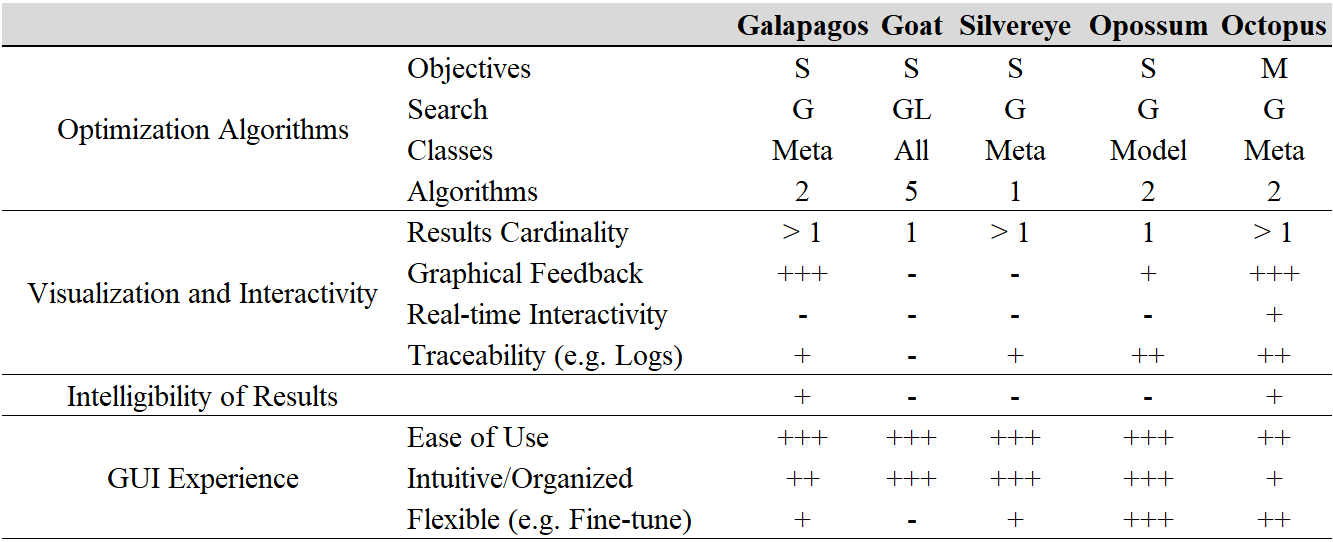
\includegraphics[width=\textwidth]{Images/Background/pluginscomparison_serif.pdf}
		\label{table:pluginscompare}	
	\end{table}
	
	When considering the interactivity and visualization mechanisms of the explored tools, all plug-ins except Goat yield multiple solutions and allow the user to re-instantiate these solutions directly in the corresponding \ac{CAD} or \ac{BIM} tool. Surprisingly, only Galapagos, Opossum, and Octopus present graphical feedback mechanisms. Particularly, Galapagos and Octopus provide not only mechanisms about the state of the optimization (e.g., parameters values being explored, current fitness values), but also an overall ranking of the best solutions. On the other hand, none of the plug-ins except for Octopus enable the user to influence and interact with the optimization process during its execution. However, even the interactions supported by Octopus are limited, consisting on the runtime modification of different configuration values (e.g., elitism, mutation, crossover operators). Regarding the traceability feature (e.g. creation of logs, solutions' lists), it is poorly supported. While Goat offers no traceability, both Galapagos and Silvereye provide a ``semi-traceable'' list with the fitness values of the best attained solutions. At last, both Opossum and Octopus support, in a way, the creation of logs describing the state of the whole optimization process, i.e., information about the evaluated design variations with their parameters and corresponding objectives values.
	
	Regarding the third aspect, there are no mechanisms explicitly designed to enhance the comprehension of the optimization results in any of the analyzed tools. However, the existence of visualization mechanisms, such as those find in Galapagos and Octopus, do enable a better understanding of the results. This understanding can be further improved by enabling the direct generation of such solutions in the corresponding 3D model, so that the user may draw conclusions by comparing different solutions. Despite the absence of visual mechanisms in Octopus, it exhibits the best solutions next to the initial solution, thus allowing the user to compare them and better understand them.
	
	Furthermore, in terms of user experience, all plug-ins are straightforward to use, requiring a single component to be added.  
	
	%One of the key differences between Goat and Galapagos is the number and diversity of the algorithms available. Whilst Galapagos supports two global metaheuristics algorithms, Goat supports five distinct algorithms: one metaheuristic, two direct-search, and two model-based algorithms, called CRS2, DIRECT, SUBPLEX, COBYLA, and BOBYQA, respectively. 
	
	% #############################################################################
	\section{Problems to Address}
	\label{sec:problemsaddress}
	
	Despite the existence of both optimization and visualization libraries, architects often lack the programming skills necessary to integrate them into an optimization process. To overcome this obstacle, 
	% Scalablity, portability, code legibility
	several optimization tools integrated in the architectural design workflow have been proposed throughout the years, as discussed in \cref{sec:optimizationtools}. In general, these tools are easy to learn and use, in part because they provide  visual programming languages. However, the visual programming paradigm often leads to scalability and program legibility issues, hence impacting the way users interact with these tools. 
	
	While the textual paradigm does not face these scalability issues, most currently existing textual \ac{AD} tools do not support optimization. Nevertheless, they already provide the mechanisms to create automated optimization processes.
	
	% Single-Objective
	An important point to consider is that, in contrast to the multi-objective view of most \ac{BPO} problems, where one aims to optimize multiple aspects simultaneously, most of the currently available optimization tools focus on \ac{SOO}. The usage of these tools to address \ac{MOO} often requires the simplification of the corresponding \ac{MOO} problem either by relaxing the objectives or by assigning preferences to each objective, as discussed in \cref{ssec:preferencesarticulation}.
	
	% Global optimization
	Another limitation of current tools is that most of them exclusively support global algorithms. While global optimization algorithms are good for obtaining close to optimal solutions, these often fail to obtain the globally optimal solutions. Instead, local algorithms can be combined with global algorithms to more rapidly converge towards the global optima. Moreover, global algorithms spend a considerable amount of time evaluating large regions of the solution space. However, if previous knowledge about the problem suggests that a global optima might be located in a certain region, a better and less time-consuming approach would be to use a local algorithm.
	
	% Unconstrained Optimization
	% Moreover, the analyzed plug-ins do not provide explicit support for hard constraints on the variables, other than the lower and upper bounds on the values of variables. While that suffices for some cases, it is not enough for many other cases in building design, where variables must relate to other according some specific relation (e.g., size of a window must be smaller than the size of the enclosing wall). 
	
	% Metaheuristic Optimization
	Also, in terms of the optimization algorithms, most tools adopt metaheuristics. While these algorithms are flexible and applicable to several domains, they lack convergence guarantees, often requiring several hundreds or thousands of evaluations to reach good results. Especially for simulation-based problems with time-consuming evaluations, this becomes a large obstacle. In the \ac{MOO} context, the situation becomes even more difficult, as the number of evaluations is multiplied by, at least, the number of objectives. This problem can be partially reduced by using model-based algorithms, where a secondary and faster model is used for evaluation, but very few tools explore this approach.
	
	% Visualization
	Regarding visualization, most tools do not provide enough visual information about the optimization state or the results themselves. In particular, most of them generate poorly formatted files with insufficient information, thus impeding any trace back to the process and even hindering the comprehension of the results, which could be achieved, for example, by associating the design parameters' configurations with the corresponding performance values. Optionally, users can produce visualization mechanisms using external tools to explore the information exported by optimization plug-ins, but this is only available in the end of the optimization run.
	
	At last, most tools do not offer the possibility for interacting with them, nor do they provide means to pause and resume optimization runs. This is an inconvenience because it prevents users from adding the knowledge they have learned during the optimization run.% users would ideally extract information from good visualization mechanisms that they could add to the process to make it more efficient.
	
	% Taking all the \textit{pros} and \textit{cons} of the analyzed tools into consideration, we identify the predominance of metaheuristics and, particularly, of evolutionary-based algorithms as one of the main drawbacks of currently existing architectural optimization tools \cite{Evins2013,Nguyen2014}, especially when considering \ac{MOO}. Due to the limitations associated with this class of algorithms and the time complexity of typical \ac{BPO} processes, the incorrect use of these algorithms might lead to slow optimization processes. Additionally, there seems to be a generalized lack of standard approach to optimization. As a result, architects tend to adopt the most easily available algorithm for every design.%, which in this case is the Galapagos' \ac{GA}. Moreover, given the difficulties and limitations of \ac{MOO}, most \ac{BPO} practitioners opt for \ac{SOO} tools. 
		
	This dissertation aims to bridge the identified gaps. To this end, we propose a framework supporting a wide variety of optimization algorithms, and providing post-processing and visual features to better support the interpretation of the optimization's results. In the next chapter, we present our solution.	
	
	% This dissertation addresses the time complexity of problems involving costly evaluation functions, especially when considering \ac{MOO}. In the next chapter, we present our solution.
	%In the next chapter, we describe the architecture of our solution and explain how each component achieves the features highlighted in this section.
		